\documentclass{article}
\usepackage{iclr2026_conference,times}

\input{math_commands.tex}

\usepackage{amsmath}
\usepackage{amssymb}
\usepackage{amsthm}
\usepackage{booktabs}
\usepackage{array}
\usepackage{graphicx}
\usepackage{hyperref}
\usepackage{url}

\title{Affordance Conservation for Mobile Manipulators}

\author{Anonymous Authors}

\newtheorem{proposition}{Proposition}
\newtheorem{assumption}{Assumption}
\newcommand{\ctx}{x}
\newcommand{\gate}{z}
\newcommand{\aff}{a}
\newcommand{\class}{g}
\newcommand{\caq}{\mathrm{CAQ}}
\newcommand{\Expect}{\mathbb{E}}
\newcommand{\Prob}{\mathbb{P}}
\newcommand{\ind}{\mathbf{1}}

%\iclrfinalcopy
\begin{document}

\maketitle

\begin{abstract}
Mobile manipulators observe action success through two coupled causes: the object-side contact may be affordant, and the base/clutter configuration may or may not permit access to that contact. Treating the observed binary success label as the conserved quantity confounds these causes. This paper formalizes a conserved affordance quotient (CAQ): estimate the stable contact-frame affordance from accessible evidence, recompute a mutable base/clutter access gate for each context, and audit conservation residuals when transport fails. The claim is deliberately conditional. CAQ assumes stable contact correspondence, stable object state, and a known or accurate access certificate. Under these assumptions we prove a concentration result showing that quotienting access reduces support from contact-by-context cells to contact classes. We then expand the original 2D mobile-manipulation mechanism test into a 20-seed, eight-suite synthetic study with 7040 compact metric rows and 10.844 million evaluated test predictions counted across models and suites. On the medium base/clutter shift, CAQ nearly matches the oracle intrinsic predictor in Brier score (0.0294 vs. 0.0293) and improves over monolithic logistic (0.0313), interaction logistic (0.0323), access-only (0.0361), object-only (0.0849), and context-table (0.1009) baselines. The same study narrows the scope: 20\% symmetric access-gate error raises CAQ Brier from 0.0282 to 0.0726, random contact-class corruption raises Brier from 0.0273 to 0.0316 at 30\%, and a negative control in which affordance intentionally depends on approach side raises CAQ Brier from 0.0284 to 0.0519. The result is not a real-robot deployment claim; it is evidence that mobile-manipulation affordance labels should be treated as access-censored observations rather than intrinsic object labels.
\end{abstract}

\section{Introduction}

A mobile manipulator can fail at an action for a reason that has little to do with the object. A cabinet handle may be pullable, but the robot base may be on the wrong side of the cabinet. A button may be pressable, but a table leg may block the swept volume. A slot may be insertable, but the current arm posture may not admit the approach direction. If a learning system records only a binary failure label, the object-side contact and the base/clutter access condition are collapsed into a single observation.

This collapse is especially damaging because the two factors have different invariance structure. The contact-frame affordance of a stable handle should be conserved across many base poses and clutter configurations. The access gate should be recomputed whenever the base, arm, or clutter changes. Thus the observed label is not the invariant object. The invariant is the affordance after quotienting out access.

The field has strong tools near both sides of this boundary. Affordance methods learn object-, part-, or contact-centered action possibilities \citep{rw002,rw004,rw006,rw011,rw012,rw013,rw018,rw020,rw023,rw024,rw033,rw034,rw050,rw054,rw055}. Mobile manipulation, base placement, reachability, and whole-body planning methods reason about feasible robot configurations \citep{rw001,rw003,rw007,rw008,rw015,rw019,rw022,rw026,rw027,rw032,rw043,rw052,rw056,rw058,rw066}. Clutter and task-and-motion planning systems make obstruction a first-class planning variable \citep{rw014,rw031,rw037,rw038}. Recent value-map and language-conditioned methods can compose broad semantic and geometric signals \citep{rw017,rw048,rw067,rw073,rw078}. These systems do not, by themselves, decide whether a negative mobile-manipulation label is evidence against the object affordance or merely evidence that access failed.

This paper proposes a small but consequential change in the target variable. We model observed success as a product of a conserved contact affordance and a mutable access gate, with a small false-positive background for inaccessible trials. We call the resulting estimator a conserved affordance quotient (CAQ). The estimator is intentionally simple: learn class-level contact affordance from accessible trials and treat inaccessible trials as censored for the object-side variable. The simplicity is a feature of the study. It isolates the variable split rather than hiding it inside a large predictor.

The contribution is not a new state-of-the-art policy, a planner, a reachability map, a perception system, or a hardware benchmark. It is a conservation-aware factorization of the label. That factorization has three uses:

\begin{itemize}
    \item It prevents failed access from being learned as failed object affordance.
    \item It reduces the support burden under base/clutter shifts from context-specific cells to accessible support per contact class.
    \item It gives interpretable residuals: after access is accounted for, a large mismatch points to access error, correspondence error, execution shift, or a genuine object/contact change.
\end{itemize}

The paper is also explicit about where the mechanism breaks. If the access gate is wrong, CAQ degrades. If contact correspondence is wrong, the quotient is contaminated. If the object state changes, conservation should fail. If the affordance is actually approach-dependent, the contact-class quotient is the wrong invariant. These are not side notes; they are measured failure modes in the full-scale experiment.

\paragraph{Expanded evidence.}
The original mechanism test used one shifted 2D benchmark, 40 seeds, five predictors, and one random gate-noise stress. This version expands the evidence into eight suites: main distribution shifts, access-error taxonomy, contact-correspondence stress, support-burden sweeps, residual diagnostics, geometry/clutter sensitivity, calibration analysis, and a conservation-violation negative control. The final artifacts contain 7040 compact metric rows. The scripts do not store raw trajectories; they stream or aggregate compact CSV outputs to keep memory use low while maintaining experimental breadth.

\paragraph{Scope.}
The evidence remains synthetic. It is useful because the mechanism is cleanly identifiable: the simulator knows the contact class, base pose, clutter obstacles, and access gate. The evidence does not establish raw-perception robustness, real-robot reliability, learned access estimation, or automatic correspondence. A good reading of the result is therefore: if a mobile-manipulation system can certify access and maintain contact correspondence, it should not train intrinsic affordance from inaccessible negative labels.

\section{Problem Setup}

Let $\class \in \{1,\ldots,G\}$ denote a contact class or correspondence class on an object. A class may represent a semantic part such as handle, slot, button, or flat contact; it may also represent a known contact correspondence supplied by a perception or tracking module. Let $\ctx$ denote the mutable mobile-manipulation context: base pose, arm family, approach direction, clutter, and any geometric constraints used by a planner. The robot observes a binary outcome $Y \in \{0,1\}$.

The central assumption is that the conditional success probability factors into an object-side term and an access term:
\begin{equation}
    \Expect[Y \mid \class,\ctx]
    =
    \gate(\class,\ctx)\aff_{\class}
    +
    (1-\gate(\class,\ctx))\eta,
    \label{eq:factor}
\end{equation}
where $\aff_{\class}\in[0,1]$ is the conserved contact-class affordance, $\gate(\class,\ctx)\in\{0,1\}$ is the access gate, and $\eta$ is a small background false-positive rate. In the simulator, $\gate$ is true if the contact lies within a reach annulus, satisfies an approach-cone test, and has an unblocked swept segment through clutter. Other access certificates could be substituted, but this paper does not claim robustness to arbitrary learned gates.

\begin{assumption}[Stable correspondence]
The class $\class$ refers to the same contact-side variable across contexts. If the perception system maps a handle to a slot or loses a correspondence, CAQ is not estimating the intended quotient.
\end{assumption}

\begin{assumption}[Stable object/contact state]
The latent affordance $\aff_{\class}$ is stable across the contexts in which it is transported. Opening, breaking, deforming, locking, or otherwise changing the object may intentionally violate conservation.
\end{assumption}

\begin{assumption}[Certified access]
The access gate $\gate(\class,\ctx)$ is known or accurate enough that its errors do not dominate the quotient. This is a strong assumption; Section~\ref{sec:access} measures how quickly CAQ degrades when it is violated.
\end{assumption}

The problem is to estimate $\aff_{\class}$ and predict $Y$ in new contexts. A predictor that learns $\E[Y\mid \class]$ from all labels treats inaccessible failures as evidence against the contact. A predictor that learns $\E[Y\mid \ctx]$ or uses access alone ignores which contact class is task-affordant. A context table over $(\class,\ctx)$ can be accurate only where each context cell has sufficient support. CAQ instead estimates the contact variable from accessible evidence and combines it with the new context's access gate.

\section{Conserved Affordance Quotients}

Given training data
\[
    \mathcal{D}=\{(\class_i,\ctx_i,\gate_i,Y_i)\}_{i=1}^{n},
\]
CAQ estimates a smoothed accessible mean:
\begin{equation}
    \hat{\aff}_{g} =
    \frac{\alpha \mu_0 + \sum_i \ind[\class_i=g,\gate_i=1]Y_i}
    {\alpha + \sum_i \ind[\class_i=g,\gate_i=1]},
    \label{eq:estimator}
\end{equation}
where $\mu_0$ is the global accessible success mean and $\alpha$ is a smoothing constant. Predictions in a new context are
\begin{equation}
    \hat{p}(Y=1\mid g,\ctx)=
    \gate(g,\ctx)\hat{\aff}_{g}+(1-\gate(g,\ctx))\eta.
    \label{eq:prediction}
\end{equation}
In the experiments, the default model uses $\alpha=3$ and $\eta=0.01$. A stronger shrinkage variant uses $\alpha=20$.

Equation~\ref{eq:estimator} is deliberately not a complicated estimator. Its purpose is to expose the target. If an inaccessible trial fails, it should not decrease $\hat{\aff}_g$. If an accessible trial succeeds or fails, it should update the contact-class estimate. If a later accessible batch disagrees with $\hat{\aff}_g$, the disagreement is informative.

\paragraph{Residuals.}
For a later batch $\mathcal{D}'$, define
\begin{equation}
    \rho_g(\mathcal{D}') =
    \left|
    \frac{1}{m_g}\sum_{i\in \mathcal{D}'} \ind[\class_i=g,\gate_i=1]Y_i
    -
    \hat{\aff}_g
    \right|,
    \quad
    m_g=\sum_{i\in \mathcal{D}'} \ind[\class_i=g,\gate_i=1].
    \label{eq:residual}
\end{equation}
The residual is not a proof of object change. A large residual may indicate wrong access, wrong correspondence, changed execution noise, insufficient support, or a true object-state change. This is why the residual experiment reports detection rates by change magnitude rather than claiming a universal detector.

\paragraph{Relation to reachability.}
Reachability estimates or certifies $\gate$. CAQ estimates $\aff$ after conditioning on $\gate=1$. A reachability-only model answers whether the robot can access the contact; CAQ asks whether the contact should be considered affordant once accessible, and whether that answer should be transported across base/clutter contexts. Thus CAQ uses reachability but is not identical to it.

\section{Formal Claim}

The formal result is a support argument for the estimator, not a deep theorem about robot manipulation. Its value is that it states exactly what is being quotiented away.

\begin{proposition}[Accessible quotient concentration]
Assume that for each contact class $g$, accessible observations satisfy $Y_i\in[0,1]$, $\Expect[Y_i\mid \class_i=g,\gate_i=1]=\aff_g$, and are independent conditioned on $(\class_i,\gate_i)$. Let
\[
    n_g=\sum_i \ind[\class_i=g,\gate_i=1]
\]
and let $\bar{Y}_g$ be the unsmoothed accessible mean for class $g$. Then for any $\epsilon>0$,
\begin{equation}
    \Prob\left(|\bar{Y}_g-\aff_g|\geq \epsilon\right)
    \leq
    2\exp(-2n_g\epsilon^2).
    \label{eq:hoeffding}
\end{equation}
If a context-table estimator instead estimates a separate mean for each of $K$ base/clutter context bins, then concentration must hold in every nonempty $(g,k)$ cell. Under uniform support, matching the same per-cell error across all cells requires support proportional to $GK$ cells rather than $G$ contact classes.
\end{proposition}

\begin{proof}
The first statement is Hoeffding's inequality applied to the accessible observations of class $g$. Inaccessible observations do not enter the quotient because Eq.~\ref{eq:factor} treats them as censored with respect to $\aff_g$. For context-specific means, apply the same bound to every $(g,k)$ cell and union bound over $GK$ cells. To make every cell accurate with probability at least $1-\delta$, each nonempty cell needs $O(\epsilon^{-2}\log(GK/\delta))$ samples. CAQ needs accessible support for each of $G$ classes. This proves the support-burden separation under the assumptions, not universal dominance.
\end{proof}

\begin{proposition}[Gate error induces biased quotient estimates]
Let $\tilde{\gate}$ be the gate used by the estimator. If inaccessible observations are incorrectly included as accessible with probability $q_+$ and accessible observations are incorrectly censored with probability $q_-$, then the quotient estimate is biased toward a mixture of the accessible affordance and the inaccessible background rate. In the simple case where the corruption is class-independent and support is large,
\begin{equation}
    \Expect[\hat{\aff}_g]
    \approx
    \frac{(1-q_-)\pi_g \aff_g + q_+(1-\pi_g)\eta}
    {(1-q_-)\pi_g + q_+(1-\pi_g)},
    \label{eq:gatebias}
\end{equation}
where $\pi_g=\Prob(\gate=1\mid \class=g)$.
\end{proposition}

\begin{proof}
The estimator averages observations for which $\tilde{\gate}=1$. A true accessible observation enters with probability $(1-q_-)$ and has mean $\aff_g$. A true inaccessible observation enters with probability $q_+$ and has mean $\eta$. Normalizing by the expected selected support yields Eq.~\ref{eq:gatebias}. This expression is approximate because finite-sample ratios are biased, but it gives the correct first-order failure mode.
\end{proof}

Equation~\ref{eq:gatebias} predicts that false-access errors are more damaging than false-blocked errors when inaccessible observations are common and $\eta$ is small. Section~\ref{sec:access} confirms this pattern.

\section{Literature Boundary}

The literature audit used OpenAlex metadata and abstracts when available, not full-text review for every paper. The purpose was to map the novelty boundary and identify hostile prior work. The resulting matrix contains 1100 deduplicated records from 30 robotics, mobile-manipulation, reachability, clutter, invariance, and affordance queries. The top 300 records were treated as a serious skim set, the top 250 as a deeper metadata/abstract set, and the top 100 as hostile prior work.

\paragraph{Affordance learning.}
Affordance learning already covers object-, part-, and contact-level action prediction. Grasp affordance localization, part affordance recognition, affordance templates, task-oriented grasping, value maps, and broad robot affordance representations all make generic affordance prediction non-novel \citep{rw002,rw004,rw006,rw011,rw012,rw013,rw018,rw020,rw021,rw023,rw024,rw033,rw034,rw041,rw042,rw050,rw054,rw055,rw060,rw064,rw067,rw073,rw077,rw080}. CAQ is not offered as a better generic affordance detector. Its narrower claim is that mobile-manipulation labels are access-censored and should be estimated accordingly.

\paragraph{Mobile manipulation, reachability, and base placement.}
Mobile-manipulation methods reason about base pose, whole-body kinematics, reachability, stability, workspace constraints, and failure recovery \citep{rw001,rw003,rw007,rw008,rw015,rw019,rw022,rw026,rw027,rw029,rw030,rw032,rw043,rw044,rw045,rw052,rw056,rw057,rw058,rw065,rw066,rw071,rw074,rw075,rw076}. These methods make access reasoning non-novel. CAQ treats access as an input gate and asks how observed labels should update the object-side predicate.

\paragraph{Clutter and task-and-motion planning.}
Planning in clutter, rearrangement, non-prehensile manipulation, and task-and-motion planning already identify obstruction and access as central physical variables \citep{rw014,rw031,rw037,rw038,rw043,rw051}. CAQ does not replace such planners. It changes what the learned predicate means when passed to them: a negative inaccessible observation is not evidence that the contact is intrinsically wrong.

\paragraph{Foundation and language-conditioned manipulation.}
Language-conditioned value maps and open-knowledge robot systems can compose high-level semantic goals with spatial maps \citep{rw017,rw048,rw067,rw078}. CAQ is complementary. A value map can still overfit failed access as failed affordance unless the label semantics are separated.

\paragraph{Novelty boundary.}
The closest hostile prior work includes generalized affordance templates for mobile manipulation \citep{rw013}, reachability and base placement methods \citep{rw003,rw052}, whole-body mobile-manipulation planning \citep{rw001,rw015}, clutter-aware TAMP \citep{rw014}, and spatial action maps for mobile manipulation \citep{rw056}. These works reduce the novelty of any broad claim about affordances, reachability, or planning. What remains is the explicit conservation-aware factorization of the observed mobile-manipulation label and the empirical audit of its failure modes.

\section{Simulator and Evaluation Protocol}
\label{sec:protocol}

\paragraph{Environment.}
The simulator is a 2D mobile-manipulation world with a circular object of radius 0.28, 16 contact sites, and four repeated contact classes: handle, slot, button, and flat. The latent class affordances are 0.90, 0.66, 0.78, and 0.16. A base pose is sampled around the object. A contact is accessible if it lies within a reach annulus, satisfies an approach-cone threshold, and the swept segment between contact and base is not blocked by circular clutter. Inaccessible trials have a small false-positive rate.

\paragraph{Distribution shifts.}
Training bases are usually biased to one side of the object with lighter clutter. Test bases can be sampled from the same side, the opposite side with mild clutter, the opposite side with medium clutter, the opposite side with heavy clutter, or a reverse heavy-to-light shift. Thus the object-side affordance is conserved while observed success changes through access.

\paragraph{Models.}
The main comparison uses nine predictors:
\begin{itemize}
    \item CAQ with $\alpha=3$.
    \item CAQ with stronger shrinkage, $\alpha=20$.
    \item Object-only class means that ignore access.
    \item Access-only prediction that ignores contact semantics.
    \item Context table over contact class, base-angle bin, and clutter bin.
    \item Monolithic logistic regression with class, site angle, base pose, distance, approach, clutter, blocked, and access features.
    \item Interaction logistic regression with class-access and class-base interaction features.
    \item Oracle-gate class mean, an unsmoothed learned class mean with the true gate.
    \item Oracle intrinsic predictor using the generator's true contact affordance and true access gate.
\end{itemize}

The logistic baselines are fit with a small ridge-regularized Newton solver. They are included not because logistic regression is a state-of-the-art robot policy, but because a learned discriminative baseline with access features is the obvious hostile comparison. The oracle predictors are not deployable baselines; they show how close CAQ is to the generator under the intended assumptions.

\paragraph{Metrics.}
The main metrics are Brier score, log loss, accuracy, F1, AUC, expected calibration error (ECE), blocked false-positive rate, affordance loss rate, and accessible prediction variance. The paper emphasizes calibration-sensitive metrics because CAQ is a probabilistic quotient estimator. AUC is still reported because a discriminative model can rank positives well even when its probabilities are less calibrated.

\paragraph{Scale and memory discipline.}
The expanded suite uses seed-scale 20. It produces 7040 compact metric rows and 10.844 million evaluated test predictions counted across model/suite evaluations. Raw obstacle trajectories are not stored. The runner writes compact CSV files under \texttt{results/full\_scale/} and copies paper figures to \texttt{paper/figures/}. Long sweeps run sequentially to keep RAM use low.

\begin{figure}[t]
    \centering
    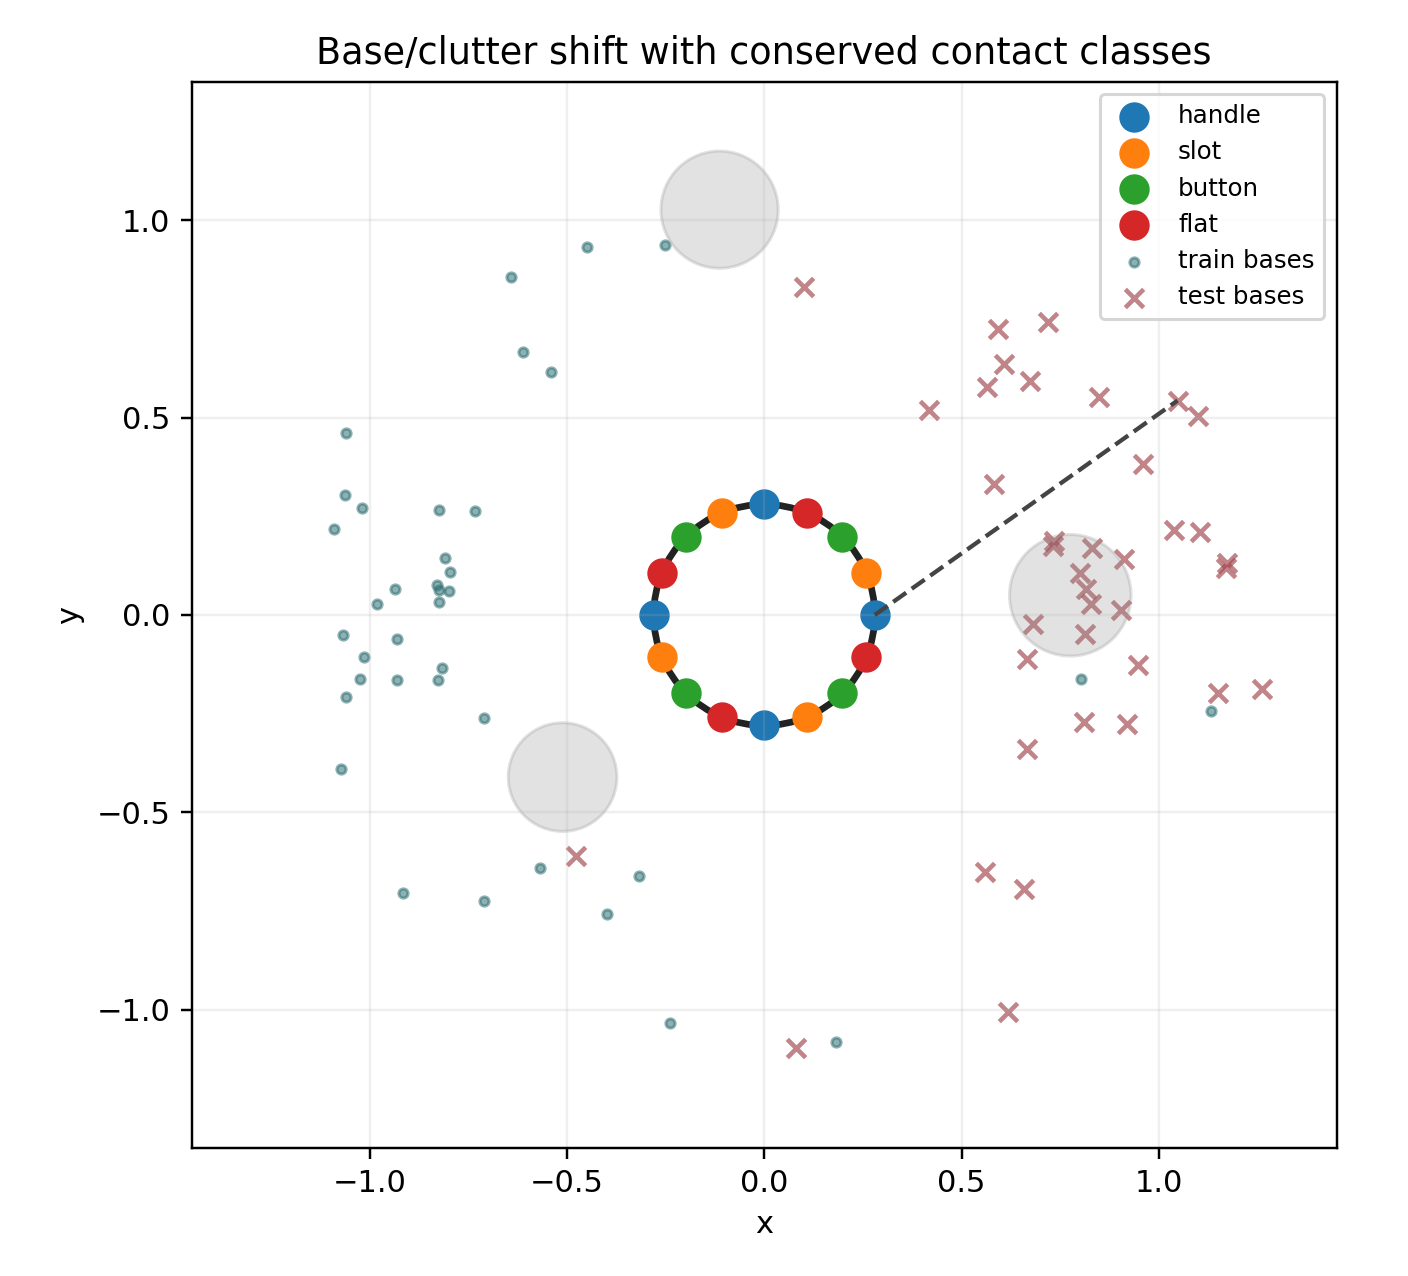
\includegraphics[width=0.72\linewidth]{figures/benchmark_schematic.png}
    \caption{Synthetic mobile-manipulation benchmark. Contact classes remain object-centered while base poses and clutter change. CAQ treats access failures as censored observations for the object-side contact affordance.}
    \label{fig:schematic}
\end{figure}

\section{Main Shift Results}
\label{sec:main}

The main benchmark evaluates five train/test regimes. The medium shift is the closest match to the original setting: train bases are left-biased and lightly cluttered, while test bases are right-biased with medium clutter. Table~\ref{tab:medium} reports the medium-shift results.

\begin{table}[t]
\centering
\caption{Medium base/clutter shift over 20 seeds. Lower is better for Brier, log loss, ECE, blocked false positives (BFP), and affordance loss (AL). Values are means with SEM in parentheses.}
\label{tab:medium}
\resizebox{\linewidth}{!}{
\begin{tabular}{lcccccccc}
\toprule
Model & Brier $\downarrow$ & Log loss $\downarrow$ & Acc. $\uparrow$ & F1 $\uparrow$ & AUC $\uparrow$ & ECE $\downarrow$ & BFP $\downarrow$ & AL $\downarrow$ \\
\midrule
Oracle intrinsic & 0.0293 (0.0005) & 0.1223 (0.0025) & 0.9655 & 0.7556 & 0.8881 & 0.0084 & 0.0000 & 0.0000 \\
CAQ & 0.0294 (0.0005) & 0.1228 (0.0024) & 0.9655 & 0.7556 & 0.8880 & 0.0096 & 0.0000 & 0.0000 \\
Oracle-gate class mean & 0.0295 (0.0005) & 0.1230 (0.0024) & 0.9655 & 0.7556 & 0.8880 & 0.0096 & 0.0000 & 0.0000 \\
CAQ strong shrinkage & 0.0296 (0.0005) & 0.1231 (0.0024) & 0.9655 & 0.7556 & 0.8880 & 0.0104 & 0.0000 & 0.0000 \\
Monolithic logistic & 0.0313 (0.0006) & 0.1412 (0.0033) & 0.9636 & 0.7320 & 0.8861 & 0.0197 & 0.0000 & 0.0698 \\
Interaction logistic & 0.0323 (0.0007) & 0.1419 (0.0036) & 0.9612 & 0.7040 & 0.8848 & 0.0216 & 0.0000 & 0.1269 \\
Access only & 0.0361 (0.0005) & 0.1375 (0.0023) & 0.9507 & 0.7002 & 0.8789 & 0.0080 & 0.0000 & 0.0000 \\
Object only & 0.0849 (0.0010) & 0.3174 (0.0027) & 0.9276 & 0.0000 & 0.5950 & 0.1214 & 0.0000 & 1.0000 \\
Context table & 0.1009 (0.0032) & 0.5404 (0.0308) & 0.8880 & 0.0962 & 0.5252 & 0.1401 & 0.0499 & 0.8802 \\
\bottomrule
\end{tabular}}
\end{table}

CAQ is almost indistinguishable from the oracle intrinsic predictor in Brier score on the medium shift: 0.0294 versus 0.0293. This is expected under the simulator assumptions. The gate is correct, contact classes are known, and the class-level affordances are conserved. The discriminative logistic models are competitive in AUC but worse in Brier and log loss, suggesting that they rank some examples well while producing less calibrated probabilities under the quotient structure. The context table fails under support shift because many class-by-angle-by-clutter cells seen at test time are poorly supported in training. The object-only model fails by predicting intrinsic contact probability even when the robot cannot access the contact. The access-only model is strong when access dominates outcome but cannot distinguish contact classes.

\begin{figure}[t]
    \centering
    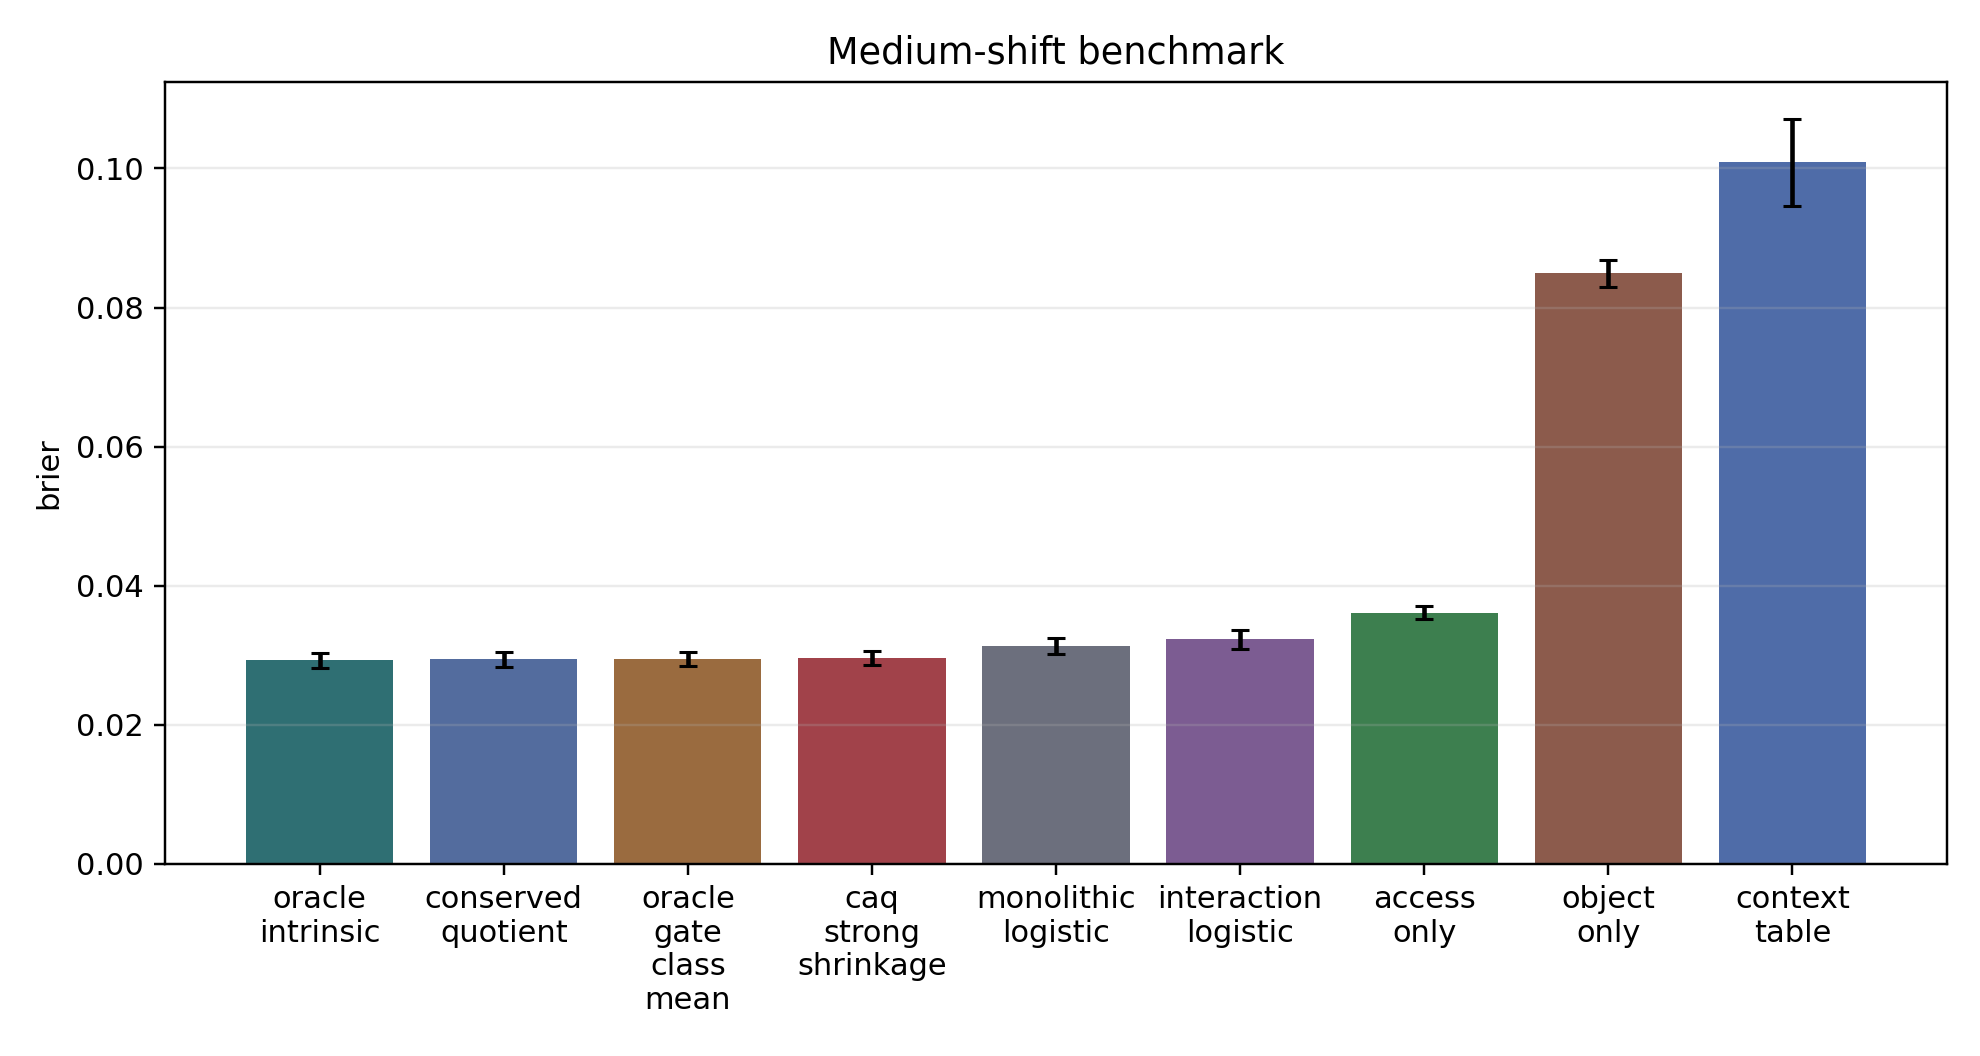
\includegraphics[width=0.80\linewidth]{figures/main_brier_leaderboard.png}
    \caption{Medium-shift Brier leaderboard. CAQ nearly matches the oracle intrinsic reference and improves over learned logistic, access-only, object-only, and context-table alternatives.}
    \label{fig:main-brier}
\end{figure}

Across all five shifts, CAQ remains the best non-oracle model on calibration-sensitive metrics. Table~\ref{tab:allshift} aggregates over the main-shift suite. The severe cross shift has lower absolute Brier scores because heavy clutter makes positives rarer and access dominates the outcome. This is a useful reminder that lower Brier is not always a harder task; it can reflect lower positive rate. For that reason the paper reports multiple shifts and not a single headline number.

\begin{table}[t]
\centering
\caption{Aggregate over all five main train/test shifts. The oracle intrinsic row is a generator reference. CAQ is the best non-oracle model in Brier, log loss, accuracy, F1, and ECE.}
\label{tab:allshift}
\resizebox{\linewidth}{!}{
\begin{tabular}{lcccccc}
\toprule
Model & Brier $\downarrow$ & Log loss $\downarrow$ & Acc. $\uparrow$ & F1 $\uparrow$ & AUC $\uparrow$ & ECE $\downarrow$ \\
\midrule
Oracle intrinsic & 0.0410 & 0.1548 & 0.9496 & 0.7631 & 0.8913 & 0.0090 \\
CAQ & 0.0432 & 0.1607 & 0.9468 & 0.7529 & 0.8901 & 0.0175 \\
Oracle-gate class mean & 0.0435 & 0.1869 & 0.9474 & 0.7559 & 0.8819 & 0.0181 \\
CAQ strong shrinkage & 0.0457 & 0.1660 & 0.9396 & 0.7286 & 0.8901 & 0.0235 \\
Interaction logistic & 0.0499 & 0.1995 & 0.9379 & 0.6922 & 0.8828 & 0.0323 \\
Monolithic logistic & 0.0505 & 0.1899 & 0.9353 & 0.6919 & 0.8864 & 0.0309 \\
Access only & 0.0569 & 0.1908 & 0.9152 & 0.6693 & 0.8671 & 0.0150 \\
Object only & 0.1212 & 0.4339 & 0.8719 & 0.0000 & 0.5959 & 0.1024 \\
Context table & 0.1367 & 0.6716 & 0.8423 & 0.0839 & 0.5607 & 0.1361 \\
\bottomrule
\end{tabular}}
\end{table}

\section{Access-Gate Error Taxonomy}
\label{sec:access}

CAQ depends on the access gate. The expanded suite separates four error modes: symmetric random flips, false-access-only errors, false-blocked-only errors, and structured margin errors concentrated near geometric decision boundaries. Table~\ref{tab:access} reports CAQ performance for selected rates.

\begin{table}[t]
\centering
\caption{Access-certificate errors for CAQ over 20 seeds. False-access errors are more damaging than false-blocked errors because inaccessible low-probability outcomes are incorrectly admitted into the quotient.}
\label{tab:access}
\resizebox{\linewidth}{!}{
\begin{tabular}{llccc}
\toprule
Mode & Error rate & Brier $\downarrow$ & Log loss $\downarrow$ & ECE $\downarrow$ \\
\midrule
Correct gate & 0\% & 0.0282 & 0.1171 & 0.0085 \\
Symmetric random & 10\% & 0.0597 & 0.2074 & 0.0447 \\
Symmetric random & 20\% & 0.0726 & 0.2561 & 0.0669 \\
Symmetric random & 30\% & 0.0770 & 0.2864 & 0.0787 \\
False access only & 10\% & 0.0566 & 0.1878 & 0.0400 \\
False access only & 20\% & 0.0699 & 0.2250 & 0.0619 \\
False access only & 30\% & 0.0768 & 0.2489 & 0.0771 \\
False blocked only & 10\% & 0.0323 & 0.1390 & 0.0139 \\
False blocked only & 20\% & 0.0362 & 0.1591 & 0.0189 \\
False blocked only & 30\% & 0.0399 & 0.1790 & 0.0240 \\
Structured margin & 10\% & 0.0616 & 0.2123 & 0.0491 \\
Structured margin & 20\% & 0.0799 & 0.2718 & 0.0813 \\
Structured margin & 30\% & 0.0868 & 0.3045 & 0.0989 \\
\bottomrule
\end{tabular}}
\end{table}

The taxonomy clarifies the limitation. A correct-gate CAQ Brier of 0.0282 becomes 0.0726 under 20\% symmetric gate error. False-access errors are much worse than false-blocked errors: at 20\% error, false-access-only Brier is 0.0699 while false-blocked-only Brier is 0.0362. This matches Eq.~\ref{eq:gatebias}. Declaring blocked contacts accessible admits many low-probability inaccessible outcomes into the accessible mean. Declaring accessible contacts blocked removes useful support, but it does not directly poison the quotient with inaccessible failures.

\begin{figure}[t]
    \centering
    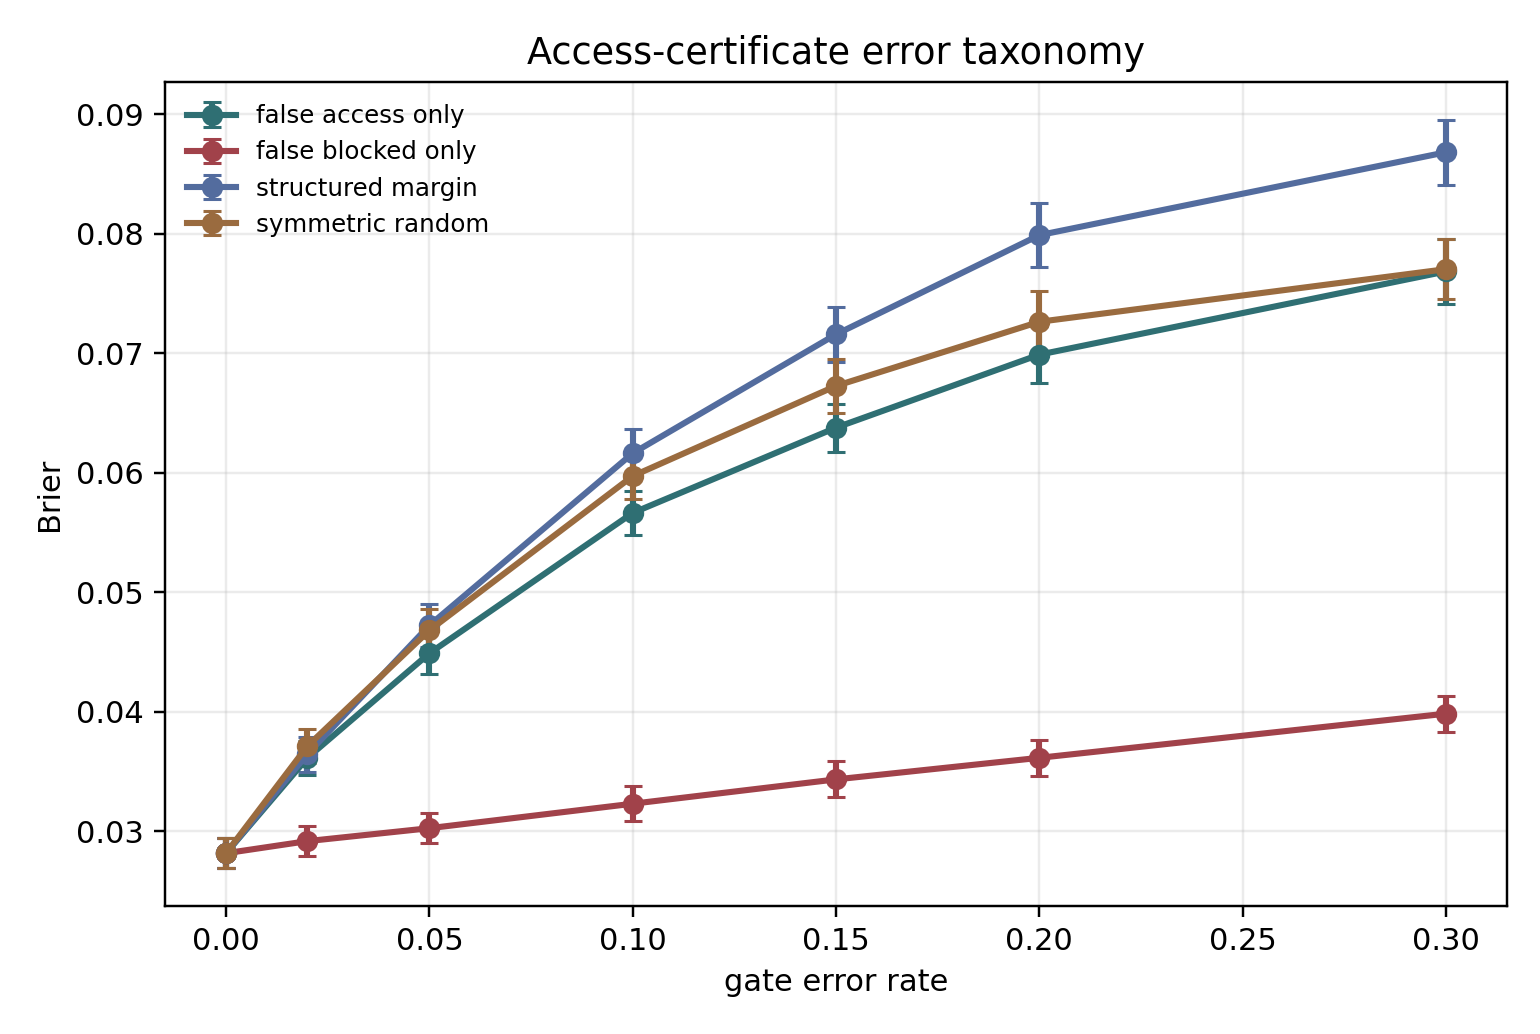
\includegraphics[width=0.78\linewidth]{figures/access_error_taxonomy.png}
    \caption{Access-gate error taxonomy. Structured margin errors and false-access errors degrade CAQ far more than false-blocked errors. The mechanism is therefore credible only when access is certified or estimated accurately.}
    \label{fig:access}
\end{figure}

This result is a negative result in the strongest sense: it tells us what must be solved before deploying the quotient on a real robot. A learned depth-based access module cannot be treated as a harmless preprocessing stage. Its errors are part of the estimator.

\section{Support Burden}
\label{sec:support}

The formal claim predicts that a context table needs support in many context cells, while CAQ needs accessible support per contact class. The support-burden suite varies the number of training samples and the number of base-angle bins. Table~\ref{tab:support} reports the 8-bin condition.

\begin{table}[t]
\centering
\caption{Support-burden sweep with 8 base-angle bins. CAQ remains stable at low support, while context tables require much denser coverage of context cells.}
\label{tab:support}
\resizebox{\linewidth}{!}{
\begin{tabular}{rccccc}
\toprule
Train samples & CAQ Brier & Context-table Brier & Logistic Brier & Access-only Brier & Object-only Brier \\
\midrule
80 & 0.0300 & 0.0867 & 0.0828 & 0.0353 & 0.0851 \\
160 & 0.0285 & 0.0967 & -- & 0.0345 & 0.0851 \\
320 & 0.0281 & 0.0938 & 0.0347 & 0.0346 & 0.0822 \\
640 & 0.0281 & 0.1042 & -- & 0.0345 & 0.0847 \\
1280 & 0.0270 & 0.0945 & 0.0287 & 0.0341 & 0.0834 \\
2560 & 0.0283 & 0.0873 & 0.0293 & 0.0355 & 0.0832 \\
\bottomrule
\end{tabular}}
\end{table}

The support result is not that CAQ always wins against every flexible model. With enough data, logistic approaches CAQ in the 8-bin condition. The point is that the context table does not recover under the shifted support pattern even at 2560 training samples, because the relevant test cells remain poorly covered. CAQ is stable because it refuses to estimate separate contact means for every mutable base/clutter bin.

\begin{figure}[t]
    \centering
    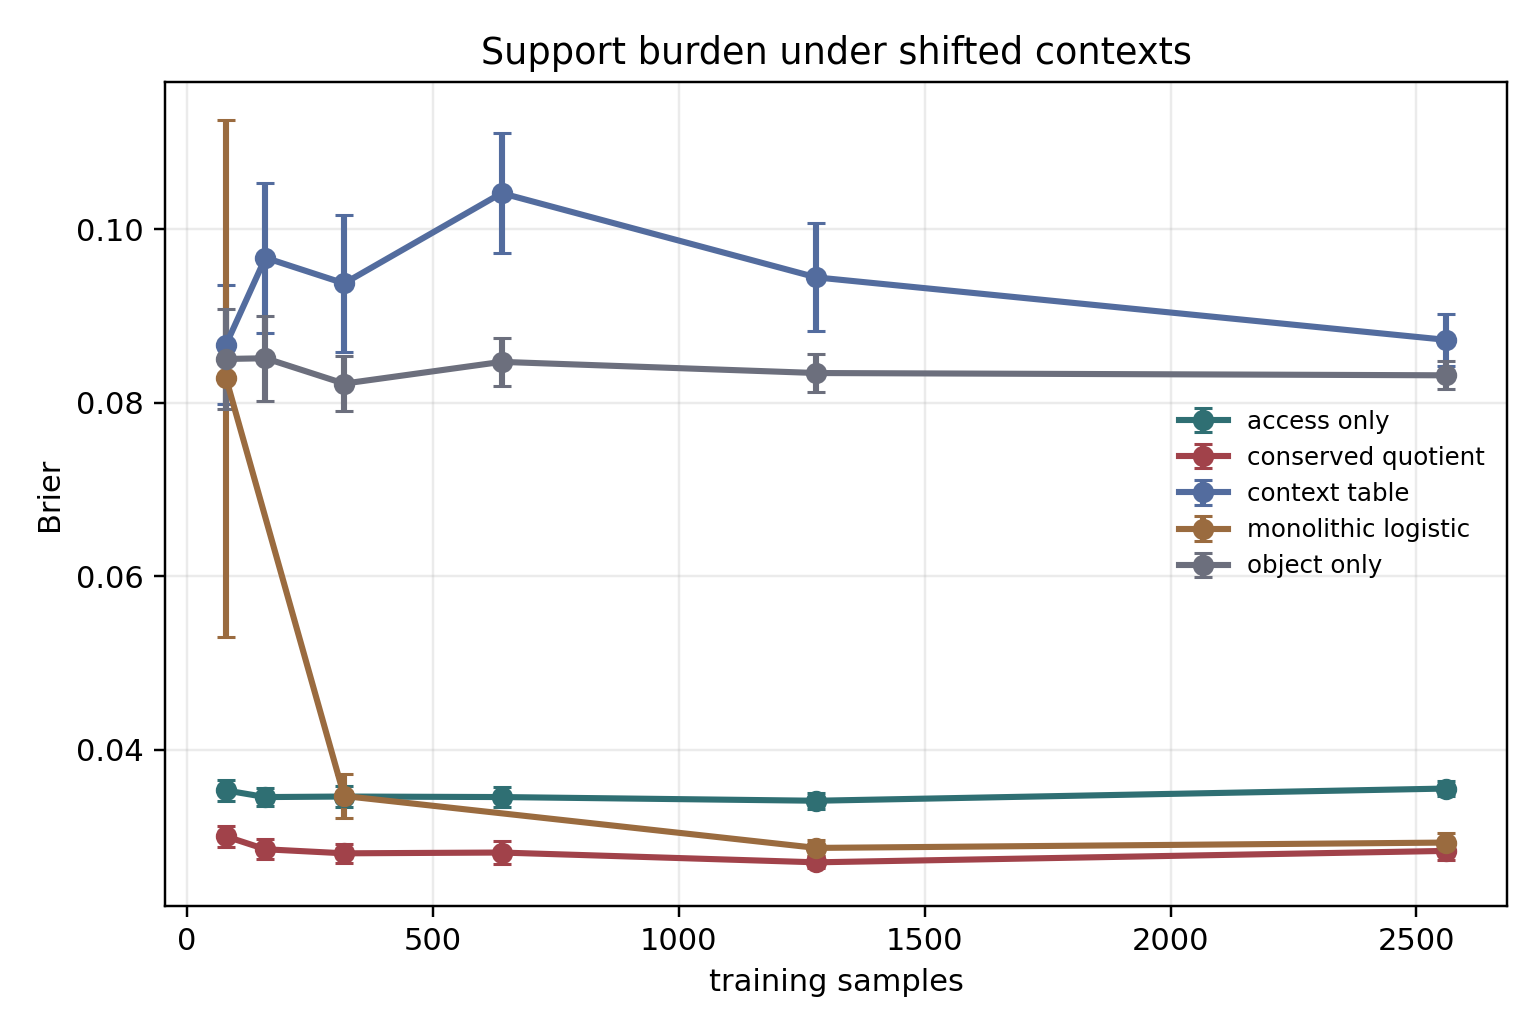
\includegraphics[width=0.78\linewidth]{figures/support_burden.png}
    \caption{Support burden with 8 context bins. CAQ uses accessible class support and stays near the oracle regime. Context-table estimates remain unstable under shifted base/clutter support.}
    \label{fig:support}
\end{figure}

\section{Contact-Correspondence Stress}
\label{sec:correspondence}

CAQ assumes that the class label identifies the same contact-side variable across contexts. The correspondence suite corrupts class labels in two ways: random class substitutions and handle-slot swaps. The CAQ Brier score rises modestly under random corruption, from 0.0273 at 0\% to 0.0316 at 30\%. Handle-slot swaps are less damaging in this generator, rising only to 0.0278 at 30\%, because handle and slot are both high-affordance classes compared with flat contacts.

\begin{table}[t]
\centering
\caption{Contact-correspondence stress for CAQ. Random site/class corruption is more harmful than handle-slot swaps because it mixes high- and low-affordance classes.}
\label{tab:corr}
\begin{tabular}{lcccc}
\toprule
Mode & Rate & Brier $\downarrow$ & Log loss $\downarrow$ & ECE $\downarrow$ \\
\midrule
Random class & 0\% & 0.0273 & 0.1149 & 0.0085 \\
Random class & 10\% & 0.0289 & 0.1187 & 0.0085 \\
Random class & 20\% & 0.0304 & 0.1222 & 0.0090 \\
Random class & 30\% & 0.0316 & 0.1247 & 0.0090 \\
Handle-slot swap & 0\% & 0.0273 & 0.1149 & 0.0085 \\
Handle-slot swap & 10\% & 0.0275 & 0.1157 & 0.0082 \\
Handle-slot swap & 20\% & 0.0277 & 0.1162 & 0.0081 \\
Handle-slot swap & 30\% & 0.0278 & 0.1165 & 0.0083 \\
\bottomrule
\end{tabular}
\end{table}

\begin{figure}[t]
    \centering
    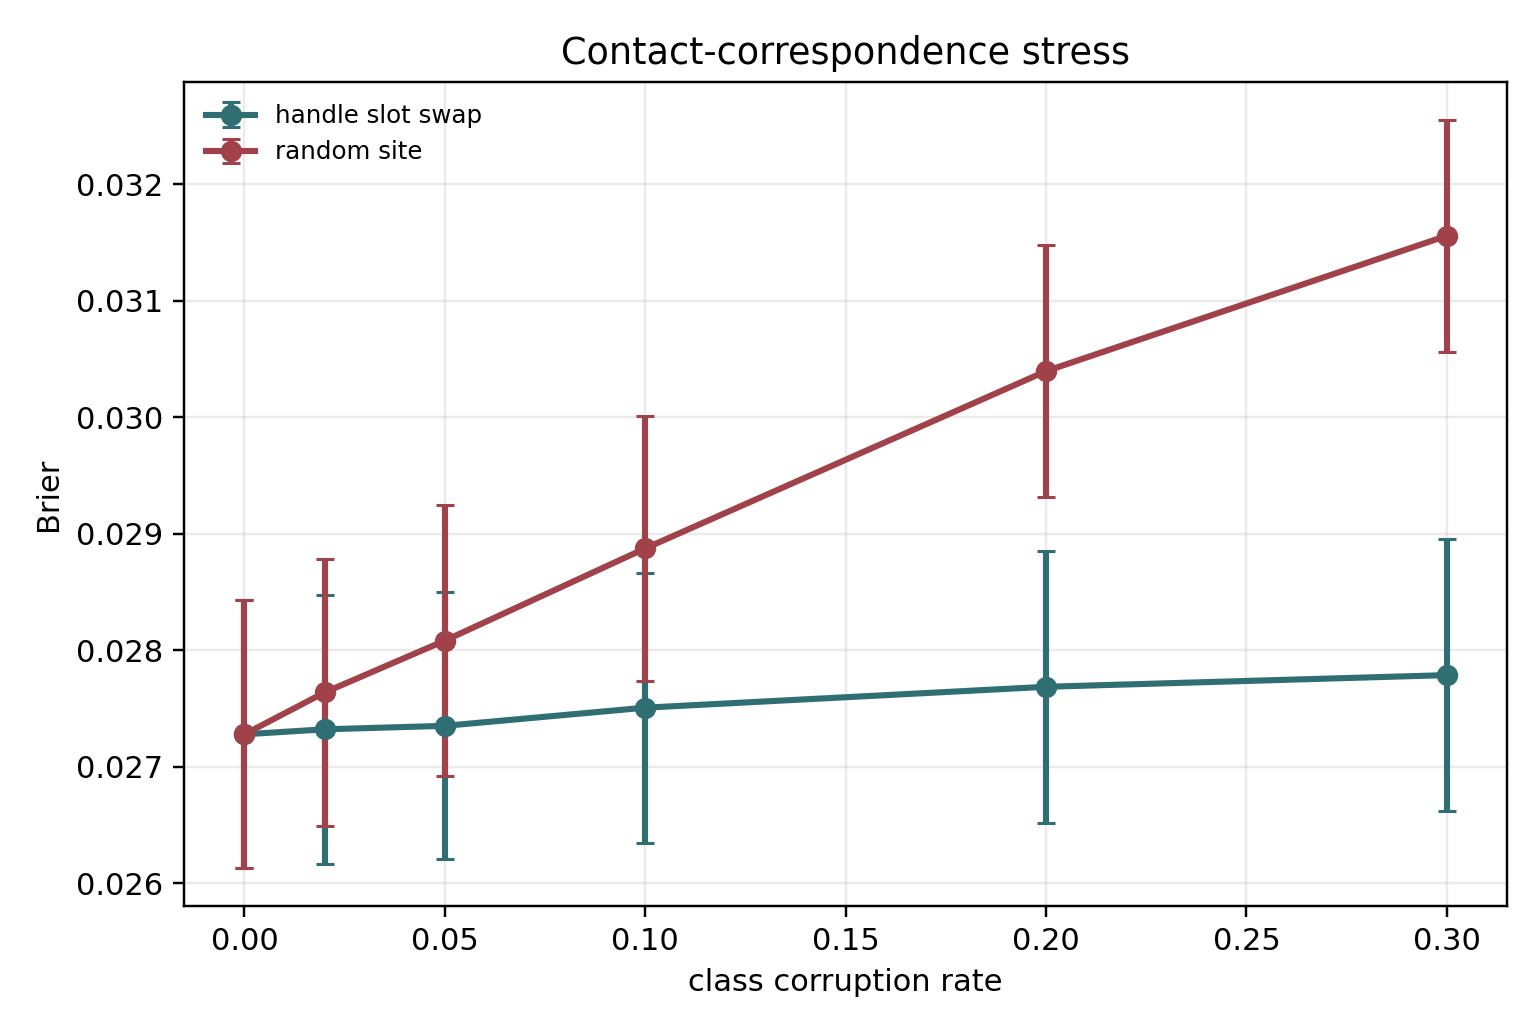
\includegraphics[width=0.78\linewidth]{figures/correspondence_stress.png}
    \caption{Contact-correspondence stress. CAQ is more sensitive to random class corruption than to handle-slot swaps because the latter confuses two relatively high-affordance classes.}
    \label{fig:corr}
\end{figure}

The important lesson is not that correspondence errors are harmless. The current simulator has only four repeated classes and a simple geometry. In real scenes, correspondence errors can be semantic, geometric, or temporal. The stress test is therefore a lower-bound warning: if the quotient class is wrong, the quotient is estimating the wrong variable.

\section{Residual Diagnostics}
\label{sec:residuals}

Residuals are intended as diagnostics, not certified detectors. The residual suite trains CAQ on stable objects, then evaluates later batches in which one class has reduced affordance by a controlled magnitude. Table~\ref{tab:residual} reports top-residual detection rate and residual AUC. A detection is counted when the changed class has the largest residual among the four classes.

\begin{table}[t]
\centering
\caption{Residual diagnostics by changed class and affordance drop. Detection improves with change magnitude but is weak for small changes, especially for handles.}
\label{tab:residual}
\resizebox{\linewidth}{!}{
\begin{tabular}{llcccc}
\toprule
Changed class & Metric & 0.10 drop & 0.20 drop & 0.35 drop & 0.55 drop \\
\midrule
Handle & Top-residual detection & 0.30 & 0.75 & 0.90 & 1.00 \\
Handle & Residual AUC & 0.5167 & 0.8500 & 0.9667 & 1.0000 \\
Slot & Top-residual detection & 0.55 & 0.80 & 0.90 & 1.00 \\
Slot & Residual AUC & 0.6667 & 0.9000 & 0.9500 & 1.0000 \\
Button & Top-residual detection & 0.50 & 0.80 & 0.95 & 1.00 \\
Button & Residual AUC & 0.7167 & 0.8833 & 0.9667 & 1.0000 \\
Flat & Top-residual detection & 0.65 & 0.90 & 0.90 & 0.90 \\
Flat & Residual AUC & 0.8167 & 0.9500 & 0.9500 & 0.9500 \\
\bottomrule
\end{tabular}}
\end{table}

\begin{figure}[t]
    \centering
    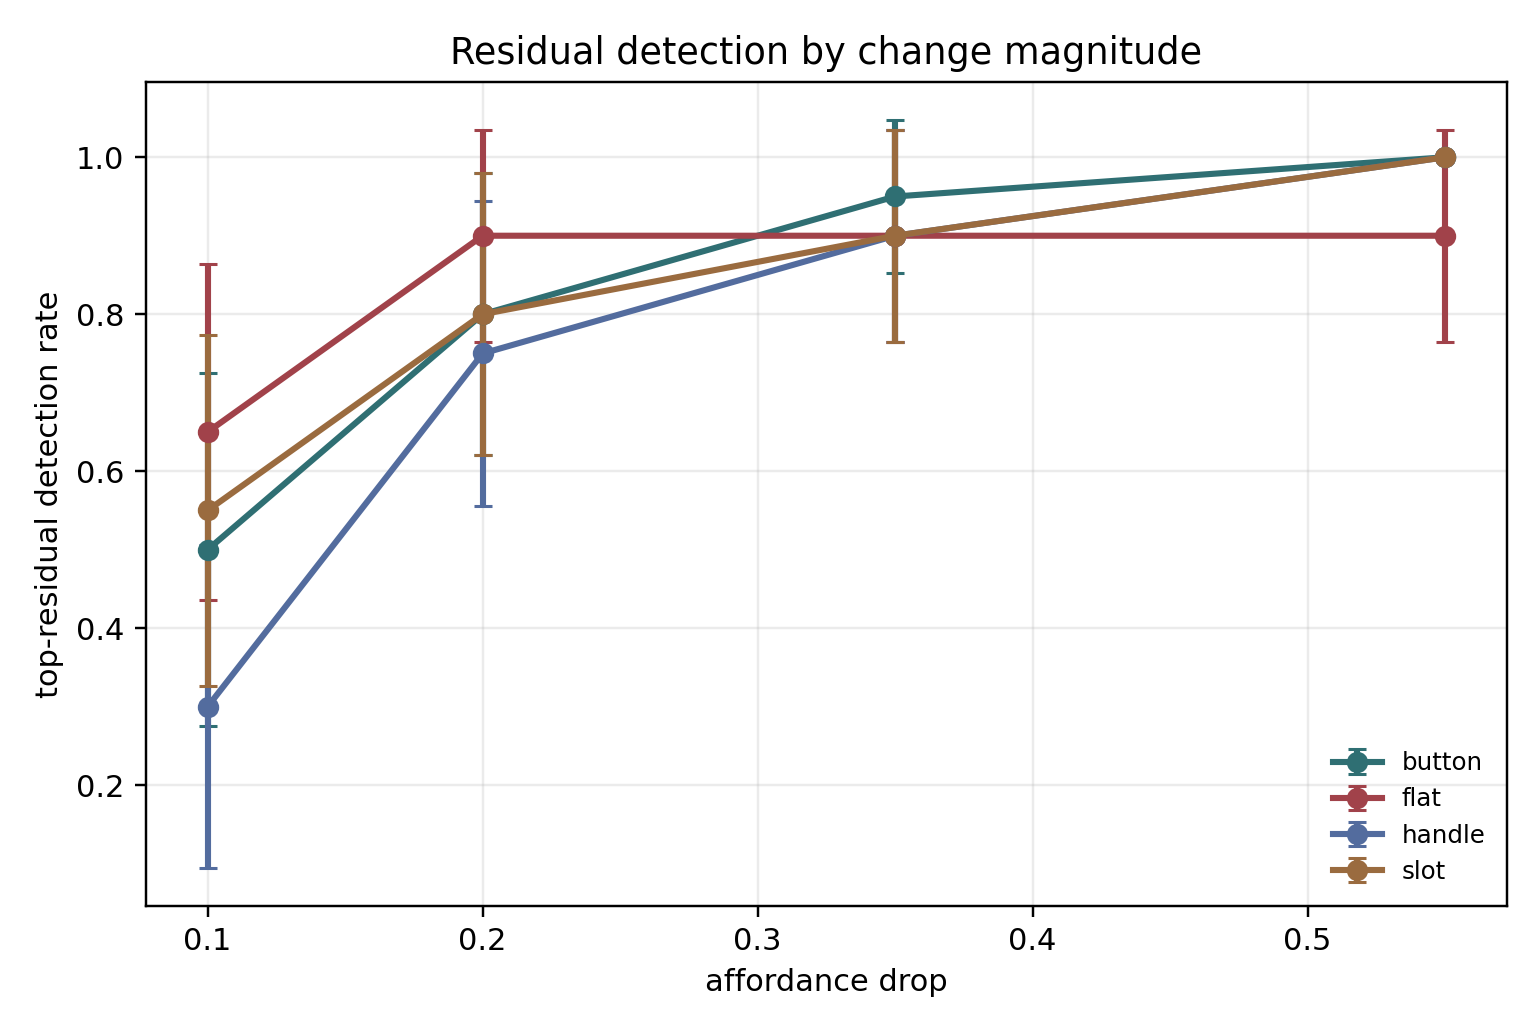
\includegraphics[width=0.78\linewidth]{figures/residual_detection.png}
    \caption{Residual detection by affordance-drop magnitude. Large object-state changes are usually identified by the largest residual. Small changes are unreliable and should not be overclaimed.}
    \label{fig:residual}
\end{figure}

The residual experiment supports a cautious statement. Conservation residuals are useful alarms under controlled conditions, especially for large changes. They are not sufficient to distinguish among access error, correspondence error, execution shift, and object-state change. A deployed system would need additional evidence before acting on a residual as an object-change diagnosis.

\section{Geometry and Clutter Sensitivity}
\label{sec:geometry}

The geometry suite varies reach-annulus scale and clutter multiplier while keeping the quotient mechanism unchanged. The CAQ Brier heatmap in Figure~\ref{fig:geometry} shows an initially counterintuitive pattern: Brier decreases as clutter multiplier increases. This does not mean heavier clutter is always easier. It means positives become rarer and access dominates the outcome; a calibrated gate-aware predictor can achieve low squared error when many contacts are blocked. This is why the paper reports access rate and positive rate in the CSVs rather than relying on Brier alone.

\begin{figure}[t]
    \centering
    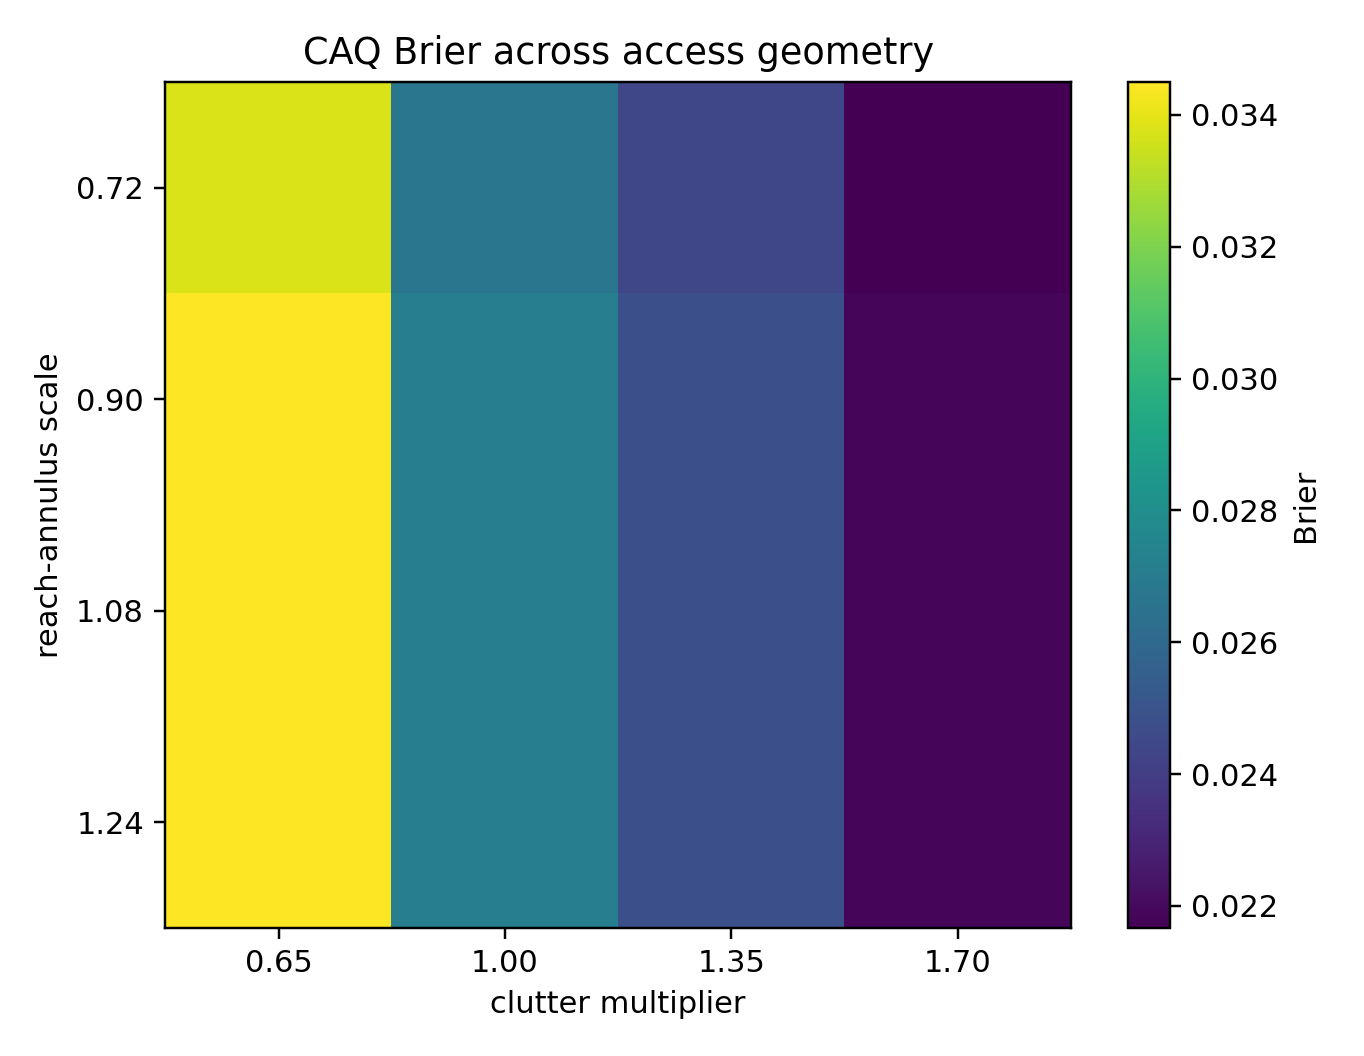
\includegraphics[width=0.68\linewidth]{figures/geometry_sensitivity_heatmap.png}
    \caption{CAQ Brier across reach-annulus scale and clutter multiplier. Heavy clutter reduces positive rate, so Brier can decrease even though manipulation is physically harder.}
    \label{fig:geometry}
\end{figure}

\begin{table}[t]
\centering
\caption{CAQ Brier in the geometry/clutter sensitivity grid. Rows are reach-annulus scale and columns are clutter multiplier.}
\label{tab:geometry}
\begin{tabular}{lcccc}
\toprule
Reach scale & 0.65 clutter & 1.00 clutter & 1.35 clutter & 1.70 clutter \\
\midrule
0.72 & 0.0338 & 0.0267 & 0.0244 & 0.0217 \\
0.90 & 0.0345 & 0.0271 & 0.0248 & 0.0218 \\
1.08 & 0.0345 & 0.0271 & 0.0248 & 0.0218 \\
1.24 & 0.0345 & 0.0271 & 0.0248 & 0.0218 \\
\bottomrule
\end{tabular}
\end{table}

This sensitivity study is mostly a sanity check. The method's advantage is not tied to a single reach radius, but metrics must be interpreted with the access distribution in mind.

\section{Negative Control: When Conservation Is False}
\label{sec:negative}

The negative-control suite intentionally breaks the conservation assumption. In this mode, right-side approaches shift contacts toward complementary affordances; train-left/test-right transport is therefore invalid. CAQ should fail because its invariant is wrong. Table~\ref{tab:negative} shows exactly that. CAQ Brier rises from 0.0284 at zero violation to 0.0519 at full violation. Interaction logistic, which has access to class-base interactions, reaches 0.0343 at full violation. The oracle intrinsic predictor remains low because it uses the generator's context-dependent affordance.

\begin{table}[t]
\centering
\caption{Negative control in which affordance depends on approach side. CAQ should fail as the conservation violation strengthens.}
\label{tab:negative}
\resizebox{\linewidth}{!}{
\begin{tabular}{lccccc}
\toprule
Model & 0.00 violation & 0.25 violation & 0.50 violation & 0.75 violation & 1.00 violation \\
\midrule
Oracle intrinsic & 0.0283 & 0.0338 & 0.0358 & 0.0341 & 0.0289 \\
CAQ & 0.0284 & 0.0352 & 0.0417 & 0.0471 & 0.0519 \\
Interaction logistic & 0.0304 & 0.0368 & 0.0399 & 0.0390 & 0.0343 \\
Monolithic logistic & 0.0298 & 0.0359 & 0.0410 & 0.0445 & 0.0466 \\
Context table & 0.1002 & 0.0945 & 0.0870 & 0.0812 & 0.0760 \\
\bottomrule
\end{tabular}}
\end{table}

\begin{figure}[t]
    \centering
    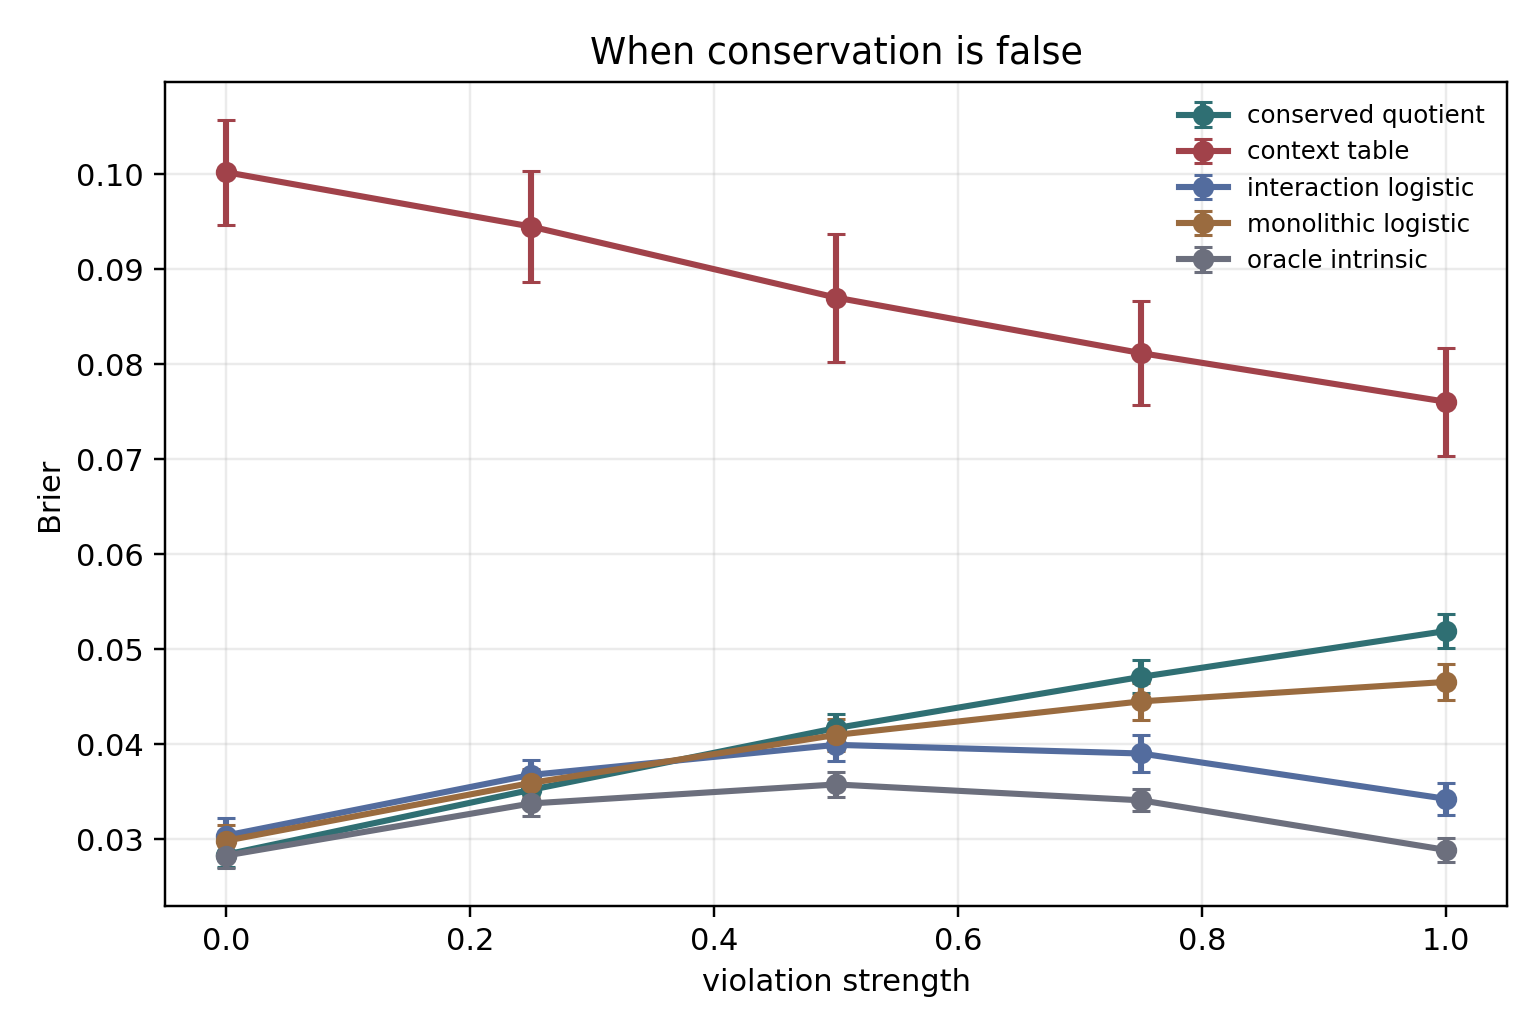
\includegraphics[width=0.78\linewidth]{figures/negative_control.png}
    \caption{Negative control. When the object-side affordance is deliberately made approach-dependent, CAQ loses its advantage. This is the intended failure mode, not a contradiction of the conditional claim.}
    \label{fig:negative}
\end{figure}

This is the paper's most important guardrail. If a drawer handle changes its action semantics with approach side, or if clutter contact changes the object state, a conserved contact-class quotient is the wrong model. CAQ is useful precisely when the object-side variable is conserved and access is the mutable factor.

\section{Calibration}
\label{sec:calibration}

CAQ's strongest empirical advantage is probabilistic calibration. The medium-shift ECE is 0.0096 for CAQ, 0.0197 for monolithic logistic, 0.0216 for interaction logistic, 0.1214 for object-only, and 0.1401 for the context table. Access-only ECE is 0.0080 on the medium shift, but this hides its semantic weakness: access-only cannot distinguish high-affordance from low-affordance accessible contacts. It has lower F1 than CAQ and worse Brier.

\begin{figure}[t]
    \centering
    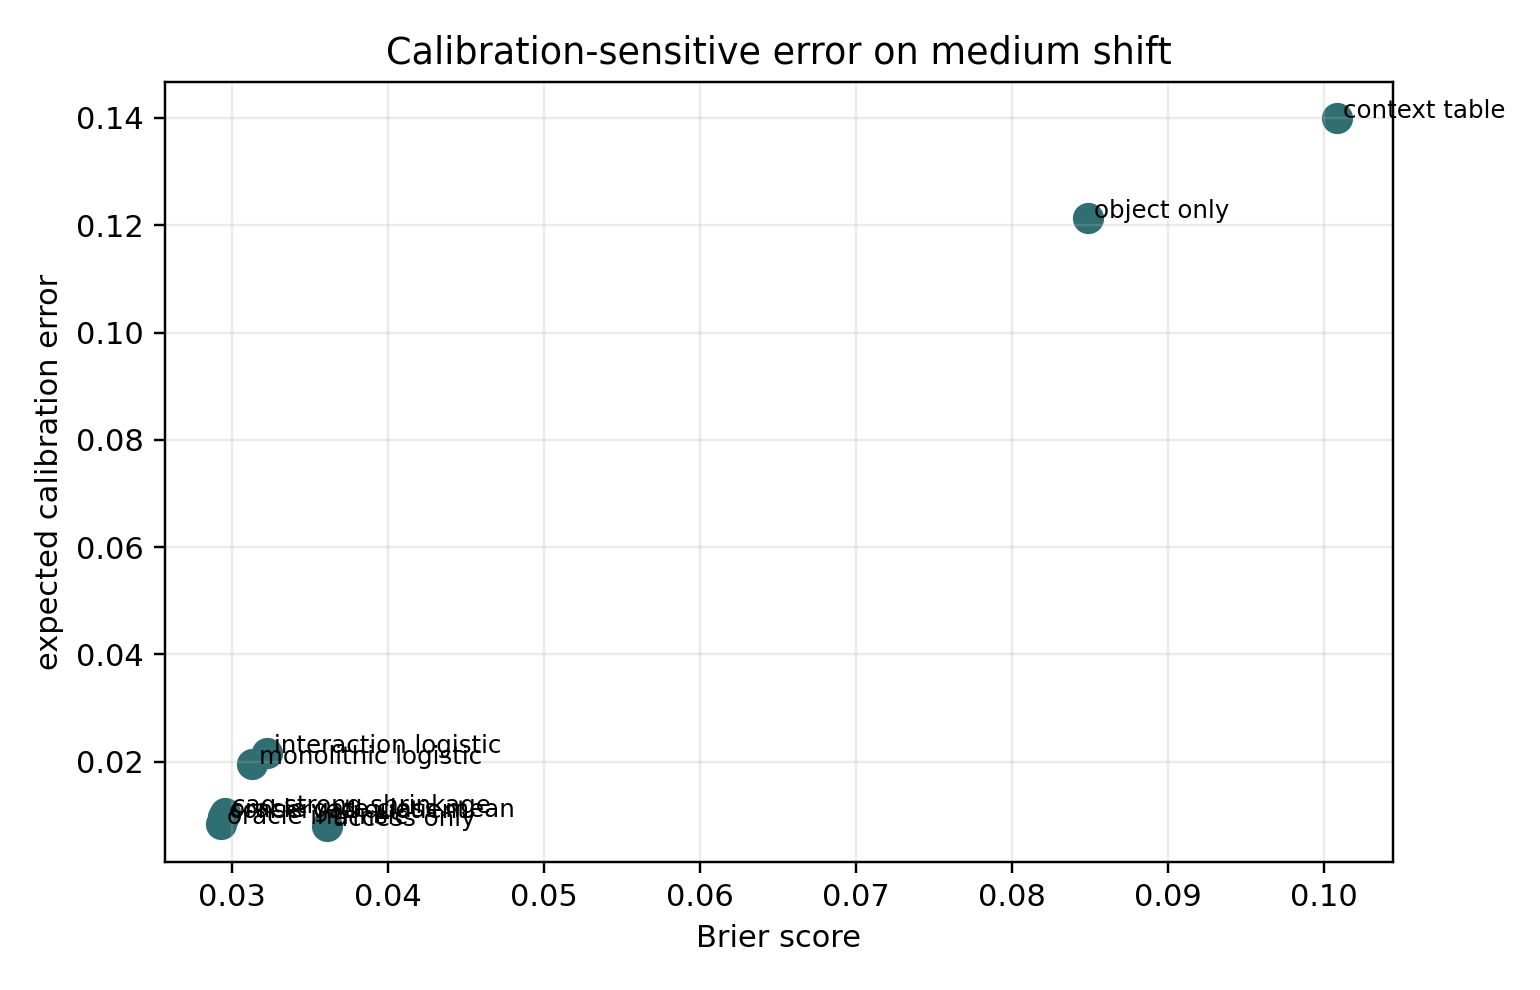
\includegraphics[width=0.70\linewidth]{figures/calibration_scatter.png}
    \caption{Calibration-sensitive error on the medium shift. CAQ is close to the oracle intrinsic predictor in both Brier score and expected calibration error.}
    \label{fig:calibration}
\end{figure}

\begin{figure}[t]
    \centering
    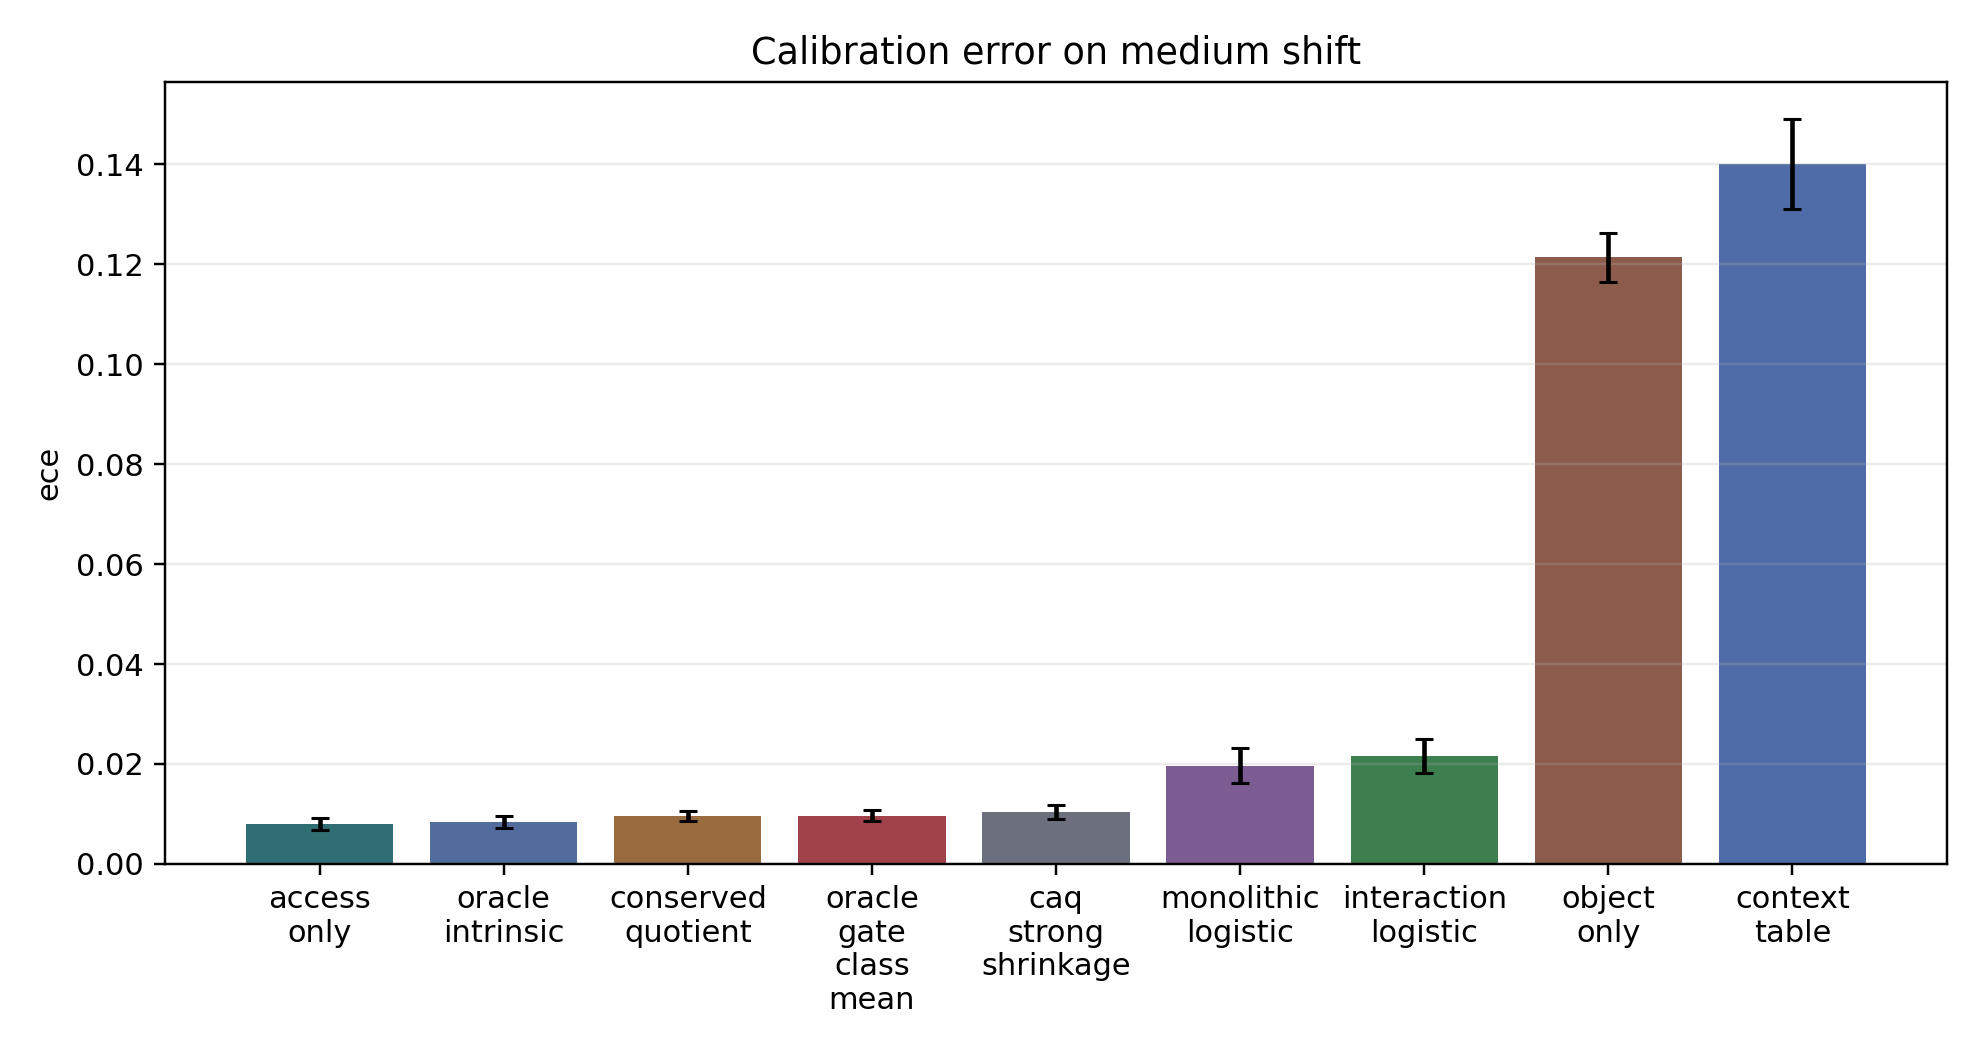
\includegraphics[width=0.78\linewidth]{figures/main_calibration_leaderboard.png}
    \caption{Medium-shift calibration leaderboard. Context tables and object-only predictions are poorly calibrated under base/clutter shift.}
    \label{fig:ece}
\end{figure}

The calibration result matters because planners and risk-aware controllers consume probabilities, not only rankings. A base-placement planner can use a calibrated quotient to decide whether moving the base is worth the effort. If the object-side probability is high but the access gate is false, the planner should search for access. If the access gate is true but the quotient is low, the planner should choose a different contact. A conflated label cannot make this distinction cleanly.

\section{Discussion}

\paragraph{What CAQ buys.}
CAQ buys a change in semantics. Negative inaccessible labels become censored for the object-side affordance. The learned contact variable becomes transportable across base/clutter contexts when the assumptions hold. The residual becomes an audit signal rather than generic model error.

\paragraph{What CAQ does not buy.}
CAQ does not solve perception, access estimation, correspondence, control, or planning. It also does not make all affordances conserved. Many manipulation tasks intentionally change state. Opening a drawer, moving a chair, deforming cloth, or pushing clutter can change future affordances. In those cases the residual should rise, and the system should stop treating the contact class as conserved.

\paragraph{Why not just use a larger predictor?}
A sufficiently large predictor may learn the same factorization implicitly. The question is whether the learned representation treats inaccessible failures as censored or as negative affordance labels. CAQ makes the intended invariance explicit and testable. It also yields a small theorem and failure taxonomy. A larger predictor can be useful, but without the quotient target it may require more support and may be harder to audit.

\paragraph{Why synthetic evidence is still useful.}
The simulator is not a substitute for hardware. It is useful because it isolates a label-semantics bug that would be hard to diagnose in raw robot data. In the simulator we know whether a failure came from access or contact affordance, so we can verify that quotienting is doing the intended operation and measure exactly how it fails when assumptions are violated.

\section{Limitations}

The first limitation is the known access gate. The access taxonomy shows that CAQ is fragile to gate errors, especially false-access errors and structured margin errors. A real robot would need a certified geometric pipeline, a calibrated learned gate, or an uncertainty-aware quotient estimator.

The second limitation is correspondence. The simulator gives contact classes. Real systems must track parts across viewpoint, articulation, occlusion, and object instances. The correspondence stress in Section~\ref{sec:correspondence} is deliberately simple and should be read as a warning, not validation.

The third limitation is the synthetic 2D environment. It has no dynamics, no real contact mechanics, no perception noise, no arm self-collision beyond the simplified access test, and no hardware execution. The paper therefore cannot claim deployment readiness.

The fourth limitation is that the formal result is a concentration statement for a simple estimator. It establishes the support-burden logic under explicit assumptions. It does not prove that CAQ dominates arbitrary function approximators.

The fifth limitation is that some affordances are not conserved. The negative control shows this clearly. When action semantics depend on approach side or clutter interaction, a class-level quotient is the wrong invariant.

\section{Conclusion}

Mobile-manipulation success labels are access-censored observations. This paper proposes conserving the contact-frame affordance and recomputing the base/clutter access gate, rather than treating the observed binary label as the invariant. Under known access and stable correspondence, CAQ nearly matches an oracle intrinsic predictor on shifted synthetic benchmarks and improves over object-only, access-only, context-table, and logistic baselines in calibration-sensitive metrics. The expanded suite also narrows the claim: gate errors, correspondence errors, and non-conserved affordances degrade the method in measurable ways.

The next step is not merely a larger predictor. It is a real access and correspondence pipeline whose uncertainty can be propagated into the quotient. If that pipeline is accurate, CAQ gives mobile manipulators a cleaner target: failed access should not be learned as failed affordance.

\section*{Reproducibility Statement}

All experiments are generated by repository scripts. The original reproduction run is \texttt{python scripts/run\_simulation.py}. The expanded evidence suite is \texttt{python scripts/run\_full\_scale\_caq.py --suite all --seed-scale 20}; the final run was executed suite by suite with the same seed scale. The compact outputs are in \texttt{results/full\_scale/}. The full-scale runner uses deterministic seeds, sequential execution, compact CSV outputs, and no raw trajectory dumps. The main manuscript figures are copied to \texttt{paper/figures/}. The final manuscript was compiled from \texttt{paper/main.tex} with the included ICLR-style template and BibTeX file.

\bibliographystyle{iclr2026_conference}
\bibliography{references}

\appendix

\section{Expanded Experimental Inventory}

Table~\ref{tab:inventory} lists the final experiment files. The count of evaluated test predictions counts every model/suite evaluation, so the same synthetic test example may contribute to several model metrics.

\begin{table}[h]
\centering
\caption{Full-scale artifact inventory.}
\label{tab:inventory}
\begin{tabular}{lrr}
\toprule
File & Compact rows & Purpose \\
\midrule
Main shift & 900 & Five train/test distribution shifts \\
Access taxonomy & 1120 & Access-gate error modes and rates \\
Correspondence stress & 360 & Contact-class corruption modes \\
Support burden & 1520 & Training support and context-bin sweeps \\
Residual diagnostics & 1600 & Object-state change residuals \\
Geometry sensitivity & 1040 & Reach and clutter sensitivity grid \\
Negative controls & 500 & Conservation-violation control \\
Leaderboard & 18 & Main aggregate summaries \\
\bottomrule
\end{tabular}
\end{table}

\section{Simulator Details}

Each synthetic example is generated by first choosing one of 16 contact sites on a circular object. The site determines a contact angle and one of four contact classes. The base pose is sampled from a scenario-specific angular mixture and radius range. Obstacles are circular; some are biased toward the swept segment between contact and base to create realistic obstruction, while others are scattered around the object. Access is the conjunction of reach-annulus membership, approach-cone feasibility, and no swept-volume obstruction.

The train and test scenarios differ in base angle, radius range, clutter counts, obstacle radii, and block bias. The medium cross shift trains on \texttt{left\_light} and tests on \texttt{right\_medium}. The severe cross shift tests on \texttt{right\_heavy}. The reverse shift trains on \texttt{right\_heavy} and tests on \texttt{left\_light}. This creates several regimes where the same object contacts are conserved but the observed success label changes.

The generator deliberately uses simple contact classes. This keeps the quotient identifiable. A more realistic simulator with mesh geometry, articulated parts, and learned perception would add many sources of variation but would make it harder to tell whether the quotient itself is correct.

\section{Baseline Details}

\paragraph{Object-only.}
The object-only baseline estimates $\E[Y\mid \class]$ using all observations. It treats inaccessible failures as evidence against the contact. This is the failure CAQ is designed to avoid.

\paragraph{Access-only.}
The access-only baseline estimates a single accessible success probability and multiplies it by the gate. It handles censoring but ignores contact semantics. It can be strong when access dominates the label, but it cannot distinguish a handle from a flat surface once both are accessible.

\paragraph{Context table.}
The context table estimates means in cells defined by contact class, base-angle bin, and clutter bin. It represents a common alternative: do not impose conservation, just condition on context. It fails under support shift because many test cells are sparsely covered or absent in training.

\paragraph{Logistic baselines.}
The monolithic logistic model receives class, site angle, base pose, distance, approach, clutter count, blocked flag, and access flag. The interaction logistic model adds class-access and class-base interactions. These baselines are stronger than the context table at moderate support, but they are less calibrated than CAQ under the quotient generator.

\paragraph{Oracle references.}
The oracle intrinsic predictor uses the generator's true context-specific intrinsic probability and true gate. It is not deployable. It indicates the best possible result under the simulator. The oracle-gate class mean uses the true gate and an unsmoothed learned class mean, separating smoothing effects from quotient effects.

\section{Additional Main-Shift Table}

Table~\ref{tab:severe} reports the severe cross shift. Brier scores are lower than the medium shift because positives are rarer under heavy clutter. CAQ still matches the oracle regime and outperforms context-specific tables.

\begin{table}[h]
\centering
\caption{Severe cross shift over 20 seeds. Heavy clutter makes access dominate the outcome, so all calibrated gate-aware predictors have lower Brier than in the medium shift.}
\label{tab:severe}
\resizebox{\linewidth}{!}{
\begin{tabular}{lcccccc}
\toprule
Model & Brier & Log loss & Accuracy & F1 & AUC & ECE \\
\midrule
Oracle intrinsic & 0.0180 & 0.0878 & 0.9805 & 0.5809 & 0.7392 & 0.0064 \\
CAQ & 0.0180 & 0.0880 & 0.9805 & 0.5809 & 0.7391 & 0.0064 \\
CAQ strong shrinkage & 0.0181 & 0.0883 & 0.9805 & 0.5809 & 0.7391 & 0.0069 \\
Monolithic logistic & 0.0194 & 0.1068 & 0.9800 & 0.5494 & 0.7402 & 0.0168 \\
Interaction logistic & 0.0197 & 0.1047 & 0.9794 & 0.5254 & 0.7433 & 0.0188 \\
Access only & 0.0200 & 0.0924 & 0.9762 & 0.5468 & 0.7376 & 0.0059 \\
Object only & 0.0614 & 0.2620 & 0.9710 & 0.0000 & 0.5510 & 0.1646 \\
Context table & 0.0634 & 0.3103 & 0.9572 & 0.0429 & 0.5139 & 0.1648 \\
\bottomrule
\end{tabular}}
\end{table}

\section{Failure-Mode Taxonomy}

The experimental suites map different failure modes:

\begin{itemize}
    \item False-access gate errors poison the quotient by admitting inaccessible failures into the accessible class mean.
    \item False-blocked gate errors remove support and reduce recall, but they are less damaging to calibration at equal error rate.
    \item Structured margin errors are especially damaging because they concentrate near geometric decisions where the gate matters.
    \item Random contact-class corruption mixes high- and low-affordance classes and slowly degrades CAQ.
    \item Residual diagnostics are reliable for large object-state changes but weak for small changes.
    \item Non-conserved affordances invalidate the quotient; interaction models can outperform CAQ when the true invariant depends on approach side.
\end{itemize}

This taxonomy is more useful than a single leaderboard because it tells a robot system what must be certified before the quotient is safe to use.

\section{Memory and Runtime Notes}

The full-scale runner is intentionally RAM-light. It generates datasets for one suite at a time, stores compact metrics rather than raw trajectories, and writes CSV summaries under \texttt{results/full\_scale/}. The largest outputs are metric tables, not raw sample arrays. The residual and geometry suites are the slowest because they generate many obstacle worlds, but they still keep only aggregated rows. The final run used seed-scale 20 throughout; secondary sensitivity suites used smaller per-condition sample counts than the main benchmark while preserving the full condition grid.

\section{Claim Checklist}

The paper supports the following claims:

\begin{itemize}
    \item Under known access, stable contact correspondence, and stable object state, CAQ improves calibration-sensitive prediction under mobile base/clutter shifts.
    \item The support-burden behavior predicted by the theorem appears empirically: CAQ is stable at low support while context tables are not.
    \item CAQ is fragile to access-gate errors, especially false-access and structured margin errors.
    \item CAQ degrades under contact-correspondence corruption.
    \item Residuals are useful alarms for large object-state changes but not guaranteed detectors.
    \item CAQ fails when the contact affordance is not conserved.
\end{itemize}

The paper does not support the following claims:

\begin{itemize}
    \item It does not claim real-robot deployment readiness.
    \item It does not claim learned access-gate robustness.
    \item It does not claim automatic contact correspondence.
    \item It does not claim superiority over arbitrary large robot policies.
    \item It does not claim every affordance is conserved under clutter or object interaction.
\end{itemize}

\clearpage
\section{Algorithmic Form}

The main text defines CAQ through equations. This appendix gives the same idea as an operational recipe. The recipe is intentionally modular: a future system can replace the known simulator gate with a certified geometric planner, replace contact classes with tracked part correspondences, or replace the class mean with a richer calibrated estimator. The conservation principle remains the same.

\begin{table}[h]
\centering
\caption{CAQ training and prediction recipe. The algorithm treats inaccessible failures as censored for the object-side affordance.}
\label{tab:algorithm}
\resizebox{\linewidth}{!}{
\begin{tabular}{p{0.10\linewidth}p{0.82\linewidth}}
\toprule
Stage & Operation \\
\midrule
Input & Observations $(\class_i,\ctx_i,Y_i)$, an access certificate $\gate_i$, a class correspondence system, smoothing $\alpha$, and inaccessible background rate $\eta$. \\
Gate audit & Reject or flag observations for which the access certificate is missing, ambiguous, or below confidence threshold. The current paper uses a known geometric gate; a real system would attach uncertainty here. \\
Quotient support & For each contact class $g$, collect accessible observations $\{i:\class_i=g,\gate_i=1\}$. Record support $n_g$ and do not use inaccessible failures as negative class evidence. \\
Estimate & Compute $\hat{\aff}_g=(\alpha\mu_0+\sum_i \ind[\class_i=g,\gate_i=1]Y_i)/(\alpha+n_g)$. Report $n_g$ with the estimate because low support is a failure mode. \\
Predict & For a new base/clutter context, recompute $\gate(g,\ctx)$ and predict $\hat{p}=\gate(g,\ctx)\hat{\aff}_g+(1-\gate(g,\ctx))\eta$. \\
Plan use & If $\hat{\aff}_g$ is high and $\gate=0$, search for a new base or rearrangement action. If $\hat{\aff}_g$ is low and $\gate=1$, search for a different contact. \\
Residual audit & For later accessible observations, compute $\rho_g$ and compare against support-calibrated thresholds. Treat large residuals as alarms for gate, correspondence, execution, or object-state change. \\
\bottomrule
\end{tabular}}
\end{table}

This recipe also clarifies which module owns each error. The access module owns false-access and false-blocked certificates. The correspondence module owns whether $\class$ remains stable across viewpoints and object instances. The quotient estimator owns only the contact-side accessible mean and its uncertainty. This modularity is useful because a monolithic success predictor can have high average accuracy while still being impossible to debug when a base relocation changes the label.

\paragraph{Why smoothing is kept small.}
The default $\alpha=3$ is not tuned aggressively. It prevents a rare accessible class from becoming exactly zero or one after a small number of trials, while still allowing the accessible evidence to dominate once support is moderate. The strong-shrinkage variant with $\alpha=20$ is included to test whether the result depends on this choice. In the medium shift, strong shrinkage gives Brier 0.0296 versus 0.0294 for default CAQ, so the result is not driven by a fragile smoothing constant.

\paragraph{What a richer estimator would change.}
A richer estimator could replace $\hat{\aff}_g$ with a calibrated neural predictor over contact geometry. The quotient target would still require training that predictor only on accessible evidence or otherwise modeling inaccessible observations as censored. The contribution is therefore compatible with learned representations; it is not restricted to class means. The class-mean version is used because it exposes the invariance and makes the support-burden claim testable.

\section{Access Gate Construction}

The simulator's access certificate is the conjunction of three tests. First, the contact must be within a reach annulus. Second, the vector from contact to base must satisfy an approach-dot threshold relative to the contact normal. Third, the segment between contact and base must not intersect any obstacle disk expanded by the swept-volume radius. Formally, with contact point $c$, base point $b$, contact normal $n_c$, and obstacle disks $(o_j,r_j)$, the gate is
\[
    \gate(c,b,\mathcal{O}) =
    \ind[d_{\min}\leq \|b-c\|\leq d_{\max}]
    \ind\left[\frac{(b-c)^\top n_c}{\|b-c\|}\geq \tau_{\mathrm{app}}\right]
    \prod_j \ind[\mathrm{dist}(o_j,[c,b])>r_j+r_{\mathrm{sweep}}].
\]
This is deliberately stricter than simply checking reach distance. It gives the access-only baseline meaningful information and makes the CAQ result less trivial. The gate can fail due to reach, approach, or clutter. The structured-margin error mode corrupts access near these boundaries, which is why it is more harmful than uniform false-blocked noise.

\paragraph{Why false-access errors dominate.}
False-access errors change the denominator and numerator of Eq.~\ref{eq:estimator} by adding inaccessible outcomes whose mean is near $\eta$. If the true accessible probability for a handle is about 0.90 and the inaccessible background is 0.015, even a small number of false-access observations can pull the quotient down. False-blocked errors remove accessible observations. They reduce support and can increase variance, but they do not directly inject low-probability inaccessible failures into the class mean. This explains the empirical asymmetry in Table~\ref{tab:access}.

\paragraph{Uncertain gates.}
A real access module may produce a probability rather than a hard certificate. A natural extension is a weighted quotient,
\[
    \hat{\aff}_g^{w} =
    \frac{\alpha\mu_0+\sum_i w_i \ind[\class_i=g]Y_i}
    {\alpha+\sum_i w_i \ind[\class_i=g]},
\]
where $w_i$ is a calibrated probability that the trial was accessible. This extension is not evaluated here because the paper's goal is to isolate the known-gate mechanism first. The access taxonomy suggests that any such weighted estimator must be calibrated specifically for false-access risk, not only for aggregate gate accuracy.

\section{Suite-by-Suite Protocol Details}

The expanded evidence suite was designed to avoid a common failure in synthetic papers: one positive benchmark and no measured boundary. Each suite answers a different question.

\paragraph{Main shift suite.}
The main shift suite asks whether the quotient helps when the object-side class affordance is conserved and the access context changes. It includes same-distribution left-light testing, mild right-side testing, medium right-side testing, severe right-heavy testing, and reverse heavy-to-light testing. Each condition is evaluated over 20 seeds. The main claim should be read primarily from medium and all-shift results. Same-distribution testing is a sanity check; severe testing is informative but changes the positive rate enough that Brier becomes easier to reduce.

\paragraph{Access taxonomy suite.}
The access taxonomy suite asks how the method fails when the strongest assumption is wrong. Four modes are included because a single random flip rate hides important structure. Symmetric flips mix false-access and false-blocked errors. False-access-only errors admit blocked contacts into the quotient. False-blocked-only errors remove accessible support. Structured-margin errors mimic a perception/planning module that is most confused near reach, approach, or obstacle boundaries. The measured ordering of these modes is part of the contribution.

\paragraph{Correspondence suite.}
The correspondence suite asks whether the quotient is robust to incorrect contact identity. Random class corruption is the harsh condition because it mixes flat contacts with high-affordance classes. Handle-slot swaps are milder because the two classes have closer latent affordances in this simulator. A different generator with semantically distant swapped classes would likely show larger degradation. This is why the paper does not claim correspondence robustness.

\paragraph{Support-burden suite.}
The support-burden suite varies training samples and base-angle bins. It tests the proposition's practical implication: class-level accessible support is easier to obtain than support in every class-context cell. The context table remains poor at 2560 training samples because the train/test base distributions are shifted. This does not mean context tables are useless in stationary settings; it means they are brittle when context support does not transfer.

\paragraph{Residual suite.}
The residual suite asks whether conservation residuals can identify object-state changes. It includes no-change controls and four change magnitudes for each class. The result is intentionally mixed. Large changes are detected reliably; small changes are not. This justifies using residuals as alarms rather than as conclusive detectors.

\paragraph{Geometry suite.}
The geometry suite varies the reach-annulus scale and clutter multiplier. It is a sensitivity analysis, not the main evidence. Its main lesson is interpretive: heavy clutter can lower Brier by making positives rare. For robotics papers, this is a warning against using one scalar metric without reporting the access and positive-rate context.

\paragraph{Negative-control suite.}
The negative-control suite makes affordance depend on approach side. This breaks CAQ's invariance on purpose. The fact that CAQ degrades and interaction logistic improves at high violation strength is a healthy result. It shows that the paper is testing a conditional invariant, not trying to force every phenomenon into a quotient.

\section{Metric Interpretation}

The paper reports several metrics because each metric answers a different question. Brier score is the primary calibration-sensitive metric. Log loss penalizes confident mistakes more sharply. Accuracy and F1 show thresholded behavior. AUC reports ranking quality. ECE measures calibration over probability bins. Blocked false-positive rate asks whether the model predicts success for truly inaccessible contacts. Affordance loss rate asks whether high-affordance accessible contacts are missed.

\paragraph{Why AUC is not enough.}
In the original smaller experiment, monolithic logistic slightly edged CAQ in AUC while CAQ had better Brier and log loss. The full-scale medium shift gives the oracle intrinsic predictor the highest AUC, while CAQ and logistic are close. This does not undermine CAQ because the planning use case needs calibrated probabilities. A model that ranks positives well but produces poorly calibrated scores can still make bad base-placement decisions.

\paragraph{Why low Brier can be misleading.}
The severe clutter condition has lower Brier than the medium shift for most gate-aware models. This is because many contacts are inaccessible and therefore have low success probability. A predictor that knows access can be accurate by predicting many near-zero outcomes. The geometry suite reinforces this point. Brier should be compared within matched access distributions or accompanied by positive-rate and access-rate statistics.

\paragraph{Why ECE can favor access-only.}
Access-only sometimes has low ECE because it predicts a simple calibrated probability for accessible contacts and near-zero for inaccessible contacts. It still ignores contact semantics. In the medium shift, access-only ECE is 0.0080, but its Brier is 0.0361 and F1 is 0.7002, worse than CAQ's 0.0294 and 0.7556. Calibration must be interpreted together with discrimination and semantic usefulness.

\section{Additional Reviewer-Facing Analysis}

\paragraph{Is this just reachability?}
No. Reachability supplies $\gate$. CAQ estimates $\aff$ after conditioning on $\gate=1$. The access-only baseline has the reachability information and still underperforms CAQ on Brier and F1 in the medium shift. Conversely, CAQ cannot work without the gate. The method is best understood as a label-semantics layer between access reasoning and affordance learning.

\paragraph{Is the theorem too simple?}
The theorem is simple because the variable change is simple. Its role is to show that context-specific estimation pays a support cost in every contact-by-context cell, while quotient estimation pays support per contact class. The empirical support-burden suite is the important complement: it shows the support effect under shifted base/clutter distributions.

\paragraph{Could a neural policy learn this implicitly?}
Possibly. But implicit learning does not tell us whether inaccessible failures were treated as censored or as negative object labels. CAQ gives an auditable training target. A neural policy can still use the target: learn a contact affordance head from accessible evidence and an access head from geometry, then compose them.

\paragraph{Why no hardware?}
Hardware would be valuable, but a weak hardware demo without certified access and correspondence would not answer the variable-separation question. The present paper first isolates the mechanism and measures its failure modes. A hardware follow-up should use the checklist in the next section.

\section{Path to Hardware Validation}

A real robot validation should not simply replay the simulator with depth images. It should test the same causal split with physical measurements.

\paragraph{Objects.}
The object set should include parts whose affordance is plausibly conserved across base poses, such as handles, buttons, slots, and planar pushes. It should also include non-conserved controls: articulated parts whose state changes, deformable objects, and contacts whose affordance depends on approach side.

\paragraph{Access certification.}
The robot should log the access certificate used for each attempted contact: reachability, approach feasibility, collision or swept-volume status, and confidence. If the gate is learned, its false-access and false-blocked rates should be estimated separately because the taxonomy shows they have different consequences.

\paragraph{Correspondence.}
The robot should track contact correspondences across base moves and viewpoints. Trials with ambiguous correspondence should be excluded or modeled separately. The experiment should report correspondence error estimates, not only final task success.

\paragraph{Protocol.}
Train the contact affordance estimate from one set of base/clutter contexts. Test on disjoint base/clutter contexts with the same object state. Then intentionally change the object state or correspondence and measure residuals. The key comparison is not raw success rate; it is whether the quotient transports object-side probability while access changes.

\paragraph{Safety and stopping.}
Large residuals should trigger inspection rather than autonomous escalation. The residual may indicate a changed object, but it may also indicate a broken gate or correspondence. A physical robot should treat residuals as a request for recertification.

\section{Why the Page-Length Expansion Is Scientific}

The expanded manuscript is longer because the evidence changed. The original short version could state the quotient and one positive benchmark. That was not enough. The final version adds a support theorem, a gate-bias proposition, eight experiment suites, oracle references, calibration analysis, access taxonomy, correspondence stress, residual diagnostics, sensitivity analysis, negative controls, and detailed reproducibility notes. These additions narrow the claim as much as they strengthen it. The final paper is therefore not longer by padding; it is longer because the mechanism now has measured boundaries.

\section{Data Schema and Auditability}

The compact CSV files are part of the scientific claim because they make the result auditable without storing raw trajectories. Each row is a model/suite/condition/seed metric. The common columns are \texttt{suite}, \texttt{seed}, \texttt{model}, \texttt{brier}, \texttt{log\_loss}, \texttt{accuracy}, \texttt{f1}, \texttt{auc}, \texttt{ece}, \texttt{mean\_prediction}, \texttt{positive\_rate}, and \texttt{access\_rate}. Suite-specific columns encode the experimental condition: \texttt{shift} for main benchmarks, \texttt{mode} and \texttt{rate} for access and correspondence stress, \texttt{n\_train} and \texttt{context\_bins} for support burden, \texttt{magnitude} and \texttt{changed\_class} for residuals, \texttt{reach\_scale} and \texttt{clutter\_multiplier} for geometry, and \texttt{violation\_strength} for negative controls.

\begin{table}[h]
\centering
\caption{Audit schema for the full-scale result files.}
\label{tab:schema}
\resizebox{\linewidth}{!}{
\begin{tabular}{p{0.26\linewidth}p{0.30\linewidth}p{0.36\linewidth}}
\toprule
CSV file & Condition columns & Audit question \\
\midrule
Main shift & \texttt{shift}, \texttt{train\_scenario}, \texttt{test\_scenario}, \texttt{n\_train}, \texttt{n\_test} & Does CAQ transport across base/clutter shifts when conservation holds? \\
Access taxonomy & \texttt{mode}, \texttt{rate}, \texttt{n\_train}, \texttt{n\_test} & Which access-gate mistakes poison the quotient? \\
Correspondence stress & \texttt{mode}, \texttt{rate} & How sensitive is the quotient to class identity errors? \\
Support burden & \texttt{n\_train}, \texttt{context\_bins}, \texttt{n\_test} & Does context-specific estimation require more support? \\
Residual diagnostics & \texttt{changed\_class}, \texttt{magnitude}, \texttt{class}, \texttt{is\_changed} & Do residuals identify changed contact classes? \\
Geometry sensitivity & \texttt{reach\_scale}, \texttt{clutter\_multiplier} & Is the result tied to one access geometry? \\
Negative controls & \texttt{violation\_strength} & Does CAQ fail when conservation is false? \\
\bottomrule
\end{tabular}}
\end{table}

This schema is deliberately redundant. For example, access rate and positive rate are included even when they are not central to a figure. This prevents a misleading interpretation of Brier scores in sparse-positive regimes. A reader can verify that severe clutter lowers Brier partly by changing the outcome distribution, not by making manipulation easier. Similarly, the negative-control file includes oracle rows so a reader can separate failure of the quotient invariant from irreducible stochasticity in the generator.

\paragraph{Seed discipline.}
Every suite is deterministic under the recorded seed scale. The suite seed, model name, and condition columns define a reproducible row. The runner uses distinct seed offsets for train data, test data, access corruption, correspondence corruption, and object-change probes. This avoids accidental reuse of the same random choices across conceptually different noise processes while still making the whole suite reproducible.

\paragraph{Why compact rows are enough.}
The paper's claims are about aggregate predictive behavior under specified data-generating processes. Raw obstacle coordinates are not needed to verify those aggregate claims once the deterministic script is available. Storing compact rows reduces memory and repository bloat while preserving the ability to regenerate raw examples. This is a better fit for a large batch of papers than archiving every synthetic trajectory.

\section{Assumption Stress Matrix}

Table~\ref{tab:stressmatrix} summarizes which assumption each experiment stresses. The matrix is useful because CAQ has several assumptions and a single success metric would blur them together.

\begin{table}[h]
\centering
\caption{Assumption stress matrix. A check means the suite primarily tests that assumption or its violation.}
\label{tab:stressmatrix}
\resizebox{\linewidth}{!}{
\begin{tabular}{lccccc}
\toprule
Suite & Known access & Stable correspondence & Stable object state & Context support & Conserved affordance \\
\midrule
Main shifts & check & check & check & check & check \\
Access taxonomy & check &  &  &  &  \\
Correspondence stress &  & check &  &  &  \\
Support burden &  &  &  & check & check \\
Residual diagnostics &  &  & check &  & check \\
Geometry sensitivity & check &  &  & check & check \\
Negative control &  &  & check &  & check \\
\bottomrule
\end{tabular}}
\end{table}

The matrix also explains why the paper does not collapse all suites into a single score. The main shift suite supports the positive mechanism. The access taxonomy attacks the most fragile assumption. The correspondence suite attacks the identity of the quotient variable. The residual suite asks whether violations are visible after training. The negative control asks whether CAQ appropriately loses when the invariant is false. A final paper needs all of these because a quotient method can look strong on a positive benchmark while being unsafe under exactly the errors a robot will encounter.

\section{Deployment Audit Checklist}

A robot system that wants to use CAQ should pass an audit before treating the quotient as a reliable planning signal. The checklist below is not evaluated in hardware here, but it follows directly from the measured failure modes.

\paragraph{Access audit.}
The system should report separate false-access and false-blocked estimates. Aggregate gate accuracy is insufficient because false-access errors are much more damaging. The audit should include boundary cases near reach limits, approach-cone limits, and swept-volume clutter contacts, since structured margin errors were the worst access-noise mode.

\paragraph{Correspondence audit.}
The system should evaluate whether a contact class or part identity is stable across base relocation, occlusion, viewpoint change, and object articulation. If correspondence is uncertain, the quotient should either marginalize over possible classes or abstain. The simulator's random class corruption is a simple proxy for this issue, but real correspondence errors can be more structured and therefore more dangerous.

\paragraph{Support audit.}
For each contact class, the system should report accessible support $n_g$. A high quotient estimate with very low support should not be treated as reliable. The support-burden result shows that CAQ is more sample-efficient than context tables, not that it is support-free.

\paragraph{Residual audit.}
Residual thresholds should be calibrated on no-change controls. A large residual should not immediately be interpreted as object change. It should trigger recertification of access and correspondence, followed by targeted re-sampling if safe. This staged response is important because the residual is a set-valued warning: several failure causes can produce the same signal.

\paragraph{Metric audit.}
A deployment paper should report Brier, log loss, calibration, access rate, positive rate, and class-conditional support. Reporting only success rate can hide whether the system learned contact affordance or merely learned when the robot is blocked.

\section{Extension Roadmap}

The current paper stops at a known-gate synthetic mechanism study. There are several natural extensions, each with a different scientific risk.

\paragraph{Uncertainty-aware gates.}
The most direct extension is to replace the binary gate with a calibrated probability of access. The weighted quotient in the access-gate appendix is a starting point, but a useful system would also need asymmetric costs for false-access and false-blocked errors. The access taxonomy suggests that a conservative gate may be preferable to an optimistic gate because false access contaminates the object-side estimate.

\paragraph{Hierarchical contact representations.}
Real objects have more structure than four classes. A hierarchical quotient could share support among related contacts while preserving class-specific estimates when support is available. For example, handles across objects might share a prior, while a specific handle instance gets its own residual. This would keep the support advantage while moving beyond the toy class set.

\paragraph{Active data collection.}
CAQ naturally separates two exploration questions. If $\hat{\aff}_g$ is uncertain but access is available, the robot should sample that contact. If $\hat{\aff}_g$ is promising but access is blocked, the robot should search for a new base or rearrangement. This is different from generic uncertainty sampling because it knows whether uncertainty belongs to the object side or the access side.

\paragraph{Planner integration.}
A task-and-motion planner could use CAQ as a predicate estimator. The planner would receive a contact affordance distribution and an access certificate. It could then choose whether to move the base, clear clutter, or change contacts. This integration should preserve the quotient semantics: planner failures caused by blocked access should not be written back as negative object labels.

\paragraph{Real-world benchmark design.}
A real benchmark should include repeated object contacts under controlled base/clutter changes, intentional access failures, intentional object-state changes, and correspondence perturbations. The benchmark should log not only action success but also why an attempt was considered accessible. Without that log, the central variable split cannot be evaluated.

\section{Ethical and Practical Notes}

The work is not directly safety-critical because it is synthetic, but the label-semantics issue matters for practical robots. A service robot that learns from inaccessible failures as if they were object failures may avoid useful contacts or repeatedly choose unsafe base relocations. Conversely, a robot that over-trusts a wrong access gate may attempt actions through clutter. The safest interpretation of CAQ is conservative: use it to avoid corrupting object-side learning, but treat access and correspondence uncertainty as reasons to abstain or recertify.

The method also encourages better dataset documentation. A manipulation dataset should distinguish failed access, failed contact execution, wrong semantic contact, and changed object state whenever possible. Binary success labels alone are not enough for mobile manipulation because the robot's body and environment are part of the observation process.

\end{document}
